\documentclass[11pt]{article}
\usepackage[margin=1.1in]{geometry}
\usepackage{amsmath,amssymb}
\usepackage{graphicx}
\usepackage[section]{placeins}
\emergencystretch=1.5em
\usepackage{booktabs}
\usepackage{caption}
\usepackage[hidelinks]{hyperref}
\usepackage{url}
\usepackage{natbib}
\bibliographystyle{apalike}
\captionsetup{font=small,labelfont=bf}
\graphicspath{{../figures/}}
\setlength{\parskip}{2pt}

\title{Why Did American Student Achievement Decline?\\[4pt]
\large Verifying the Trends and Testing Competing Explanations with NAEP Data}
\author{Brendan Bartanen\\[2pt]
{\normalsize University of Virginia}}
\date{{\normalsize July 2, 2026 --- Version 2.0\\[1pt]
{\small First version: June 9, 2026 (v1.0); v1.9 (June 12, 2026) incorporated the NAEP Long-Term Trend\\ results for 2025 released June 10, 2026; v2.0 responds to a written external review.\\ Version history: GitHub releases v1.0--v2.0 at \url{github.com/brendanbartanen-svg/naep-achievement-decline}.}}}

\begin{document}
\maketitle

\begin{center}
\begin{minipage}{0.94\textwidth}
\small\noindent\textbf{How this report was produced.} This document is an experiment in AI-conducted research, and the division of labor behind it is unusual enough to state plainly rather than leave to a byline. The research and the text were produced by Claude (Fable 5), an AI model from Anthropic, over a series of interactive sessions in June 2026. The model pulled all data from federal APIs and survey microdata files, wrote and ran every analysis script, produced every figure, and drafted every sentence of this document, including this paragraph and the Limitations and Verification sections. The listed author directed and verified rather than executed: posing the initial question, choosing which directions to pursue and when to stop, supplying occasional leads from outside the sessions (most recently the June 2026 release of the 2025 Long-Term Trend results, incorporated in v1.9), carrying out the human verification steps recorded in the repository, and deciding what was release-ready. The author wrote none of the code and none of the prose. The byline follows the scholarly convention that reserves authorship for the human who takes responsibility for the work and asks that AI involvement be disclosed rather than credited; this paragraph is that disclosure.\par\medskip\noindent Version 2.0 (July 2026) responds to a written external review with claim-strength calibration, symmetric treatment of the report's two null designs (waiver timing and 4G rollout), an added rival-hypothesis analysis (adolescent mental health), and a full organizational and line-level edit, carried out under the same division of labor; no analyses, estimates, or data changed. No human has line-edited the text or re-derived the full analysis. In place of that, the project carries the layered verification record described in Section~\ref{sec:verification}: a typed audit of every load-bearing claim with a human-executable check, an assertion suite frozen against the published numbers, blind replications of the riskiest results by independent AI agents denied access to this project's code, external anchoring to published estimates, and the author's spot-checks of the hand-coded datasets and headline numbers at the scopes recorded in the repository. The repository is public, with code, data extracts, evidence files, and version history, at \url{https://github.com/brendanbartanen-svg/naep-achievement-decline}. Readers should weigh the report as what it is: machine-produced analysis with documented provenance, verified at the stated scopes and no further.
\end{minipage}
\end{center}
\vspace{2pt}

\begin{abstract}
\noindent American student achievement has fallen substantially over the past decade. Drawing directly on the National Assessment of Educational Progress (NAEP) Data Service API, this report verifies the decline and tests eight candidate explanations against its timing, distribution, subgroup incidence, geography, and international parallels. The decline has two phases. Phase one (2013--2019) was a slow erosion concentrated almost entirely among low performers: age-13 Long-Term Trend (LTT) mathematics fell 12.6 points at the 10th percentile between 2012 and 2020 while the 90th was flat. Phase two (2020--2022) was an abrupt, across-the-board pandemic drop, then a weak recovery that stalled at the bottom. By 2024, grade 8 reading was the lowest ever recorded and every 90--10 gap the widest on record; the 2025 LTT shows 9-year-olds beginning a bottom-led recovery while 13-year-olds sit at multi-decade lows. Pandemic disruption clearly caused phase two but cannot explain phase one. Chronic absenteeism, roughly doubled after 2020, is the leading brake on recovery; demographic change, funding cuts, and teacher shortages contribute little. Four discriminating tests weaken every strong school-policy account of phase one: grade 8 losses arose between grades 4 and 8 in cohorts entering at record levels; Catholic schools, never subject to federal accountability, declined in step with public schools; NCLB-waiver timing shows no detectable effect on bottom-decile scores; and Common Core never-adopters declined as much as adopters. The same bottom-concentrated decline appears among adults in nineteen OECD countries. Among the candidates examined, post-2012 smartphone and digital-media saturation of adolescent life is the explanation the tests consistently favor, with adolescent mental-health deterioration the strongest entangled rival, pending a pre-registered state phone-ban test against NAEP 2026. A county 4G-rollout event study, this project's adversarial check on its leading candidate, finds no detectable effect of local arrival timing. The result is a consistency ranking, not a causal estimate.
\end{abstract}

\section{Introduction}

For two decades beginning in the early 1990s, American students made steady, historically large gains on the National Assessment of Educational Progress (NAEP), the nation's longest-running and most credible barometer of K--12 achievement. Fourth-grade mathematics scores rose nearly a full standard deviation between 1990 and 2013. That era is over. Every major NAEP series peaked between 2012 and 2015 and has fallen since, with the steepest losses after 2019. The reversal is large: by 2024, average grade 8 mathematics scores had returned to their 2000 level, and grade 8 reading scores were the lowest ever recorded in the assessment's history.

This report does two things. First, it \emph{verifies} the decline directly from primary data, pulling national, state, percentile, and subgroup statistics from the NCES NAEP Data Service API rather than relying on secondary summaries \citep{naepapi}. Second, it \emph{tests} eight candidate explanations against five kinds of evidence: (i) the timing of the decline; (ii) its distribution across the achievement spectrum; (iii) its incidence across demographic subgroups; (iv) its geography across states; and (v) its presence or absence in other countries.

Most public discussion attributes the decline to the COVID-19 pandemic. A central finding of this report is that the pandemic explanation, while clearly correct for the 2019--2022 drop, is incomplete. Between a quarter and three-quarters of the total decline, depending on grade and subject, either predates March 2020 or postdates the return to in-person schooling. The pre-pandemic phase also has a distinctive signature that any complete explanation must fit: losses concentrated almost entirely among low performers.

How this report reasons from evidence to conclusion deserves stating up front, because it fixes what the conclusions can claim. The analysis is observational: national test-score trends admit no randomized variation, and several candidate causes operate at once. The discipline imposed is eliminative. We enumerate the candidate explanations advanced in research and public debate, derive from each one discriminating predictions across the five kinds of evidence just listed, score each hypothesis against the same set of facts, and, where usable policy or infrastructure variation exists, run direct tests or pre-register them (as with the state phone-ban test against NAEP 2026). The output is a ranking of candidate explanations by their consistency with the evidence, not a causal estimate. Consistency is a screen, not proof, and the candidate list stays open: an explanation can lead the ranking and still be wrong. The report's strongest claims are therefore negative, about which explanations the evidence rejects; the positive conclusion is a ranking, held provisionally and subject to direct tests as they arrive.

The report proceeds as follows. Section~\ref{sec:related} places the contribution in the existing literature, and Section~\ref{sec:data} describes the data. Section~\ref{sec:verify} verifies the decline and distills it into eight facts (F1--F8) that any explanation must fit. Section~\ref{sec:candidates} lists the eight candidate explanations, and Section~\ref{sec:testing} assesses each against those facts. Section~\ref{sec:sharper} reports five sharper tests built from cohort structure, school sector, and policy and rollout timing; Section~\ref{sec:mechanism} checks the phase-two channels (schooling mode, attendance) and whether falling test-taking effort could account for the measured decline. Section~\ref{sec:synthesis} assembles the scorecard and states the resulting ranking. Limitations, the verification record (Section~\ref{sec:verification}), and a short conclusion close the report.

\section{Related Work and Contribution}
\label{sec:related}

The decline itself is well documented. NCES's own releases established the 2012--2013 peak and the concentration of losses among low performers. \citet{malkus2025theories} assembles percentile trends across 21 assessments and distills four facts any explanation must fit: a $\sim$2013 onset, bottom-half concentration, internationally outsized U.S. gap growth, and parallel declines among \emph{adults} on PIAAC. Section~\ref{sec:adults} incorporates that last fact and sharpens it with the 2023 Cycle 2 results. \citet{wyckoff2025} documents the same patterns at the state level, and the Education Recovery Scorecard project has traced the pandemic shock and recovery at district scale \citep{kane2024,kane2025,dewey2026}.

The hypothesis-weighing genre is likewise established. \citet{malkus2025theories} and \citet{wyckoff2025} evaluate candidate explanations narratively against descriptive patterns, and the conclusions this report reaches on the COVID and absenteeism hypotheses rest on existing causal work \citep{goldhaber2023,jack2023,cea2023,dee2024}. The weak state-level correlation between pandemic schooling mode and NAEP changes was noted on release day in 2022 (by Chalkbeat's analysis and by the NCES commissioner; \citealp{barnum2022}) and has an academic treatment in \citet{lsae2025}; Section~\ref{sec:dose} confirms it with a pooled design and supplies the aggregation interpretation.

On the digital-media hypothesis specifically, the nearest causal antecedents sit outside the U.S. achievement literature. \citet{jainstemper2024} estimate the effect of 3G arrival on PISA scores across 82 countries, and a 2025--26 rollout-based literature traces the same smartphone shock through fertility and family formation \citep{myershooper2026,hudsonmoscoso2026}; Section~\ref{sec:h2} imports both. No within-U.S. mobile-rollout design against test scores previously existed; \citet{wyckoff2025} states the direct causal evidence is lacking. Section~\ref{sec:fourg} supplies a first pass: a county-level 4G-rollout event study built from the archived National Broadband Map, which returns a precise null on the arrival-timing margin while leaving the national and adoption margins open.

Three analyses in this report do not, to our knowledge, exist in published form, and each fills a gap that the existing literature has explicitly flagged:

\emph{First}, the waiver-timing event study (Section~\ref{sec:waiver}). \citet{dewey2026} make the descriptive observation that post-2013 declines were similar in waiver and non-waiver states, and write of the sustained-accountability counterfactual that it ``has never been tested.'' The causal waiver literature is within-state: regression-discontinuity studies of priority/focus designations in Michigan, Kentucky, and Louisiana \citep{hemeltjacob2020,deedizonross2019}. \citet{deejacob2011} identify NCLB's \emph{adoption} effects from cross-state timing of prior accountability; Section~\ref{sec:waiver} runs that design in reverse on the policy's dismantling. The closest prior empirical estimate is \citet{bleiberg2020}, whose dissertation difference-in-differences of waiver receipt (binary, by 2013) on mean student-level NAEP scores through 2013 finds no average effect, a result that corroborates ours at the mean; his published waiver work concerns school-improvement designations within waiver states \citep{bleiberg2026}. What remains distinct here is the staggered-timing-plus-never-treated design carried through 2019, the percentile outcomes that the bottom-concentrated decline makes essential, and the randomization inference with an explicit power benchmark.

\emph{Second}, the cohort/period decomposition (Section~\ref{sec:cohort}). \citet{petrilli2020} tracked two graduating classes informally and observed that their losses arose between grades 4 and 8; \citet{malkus2025theories} argues against ``cohort-cascade'' accounts narratively. Section~\ref{sec:cohort} provides the formal version: a cohort-matched decomposition of every grade 8 change into grade 4 entry and grades 4--8 growth, showing the declining cohorts arrived at record levels---the demonstration the narrative arguments lacked.

\emph{Third}, the sector test (Section~\ref{sec:sector}). \citet{malkus2015} noted after a single cycle (2013--2015) that combined public-plus-private estimates fell as much as public-only estimates and drew the same inference this report draws; Catholic-school NAEP commentary since has focused on COVID-era resilience. Section~\ref{sec:sector} executes the test systematically over the full pre-pandemic window, at the percentile level, with published-SE-based inference---navigating the fact that NAEP stopped reporting all-private results after 2013, which makes the Catholic series the only usable private benchmark.

Beyond the three tests, the report's integrative device derives distinct predictions from each hypothesis across timing, distribution, cohort structure, sector, geography, and international comparisons, and scores each hypothesis against a common set of facts. We believe this is a more disciplined version of an argument that has so far been conducted one hypothesis at a time.

\section{Data}\label{sec:data}

\paragraph{Main NAEP.} The primary data are national public- and private-school average scale scores and percentile scores (10th, 25th, 50th, 75th, 90th) for mathematics and reading at grades 4 and 8, for all assessment years from 1990 (mathematics) and 1992 (reading) through 2024, retrieved from the NAEP Data Service API \citep{naepapi}. Subgroup means (race/ethnicity, sex, National School Lunch Program eligibility), school-sector results (public, Catholic, private), state-level means for 2013--2024, and a state $\times$ year panel of percentile scores (2003--2024) come from the same source. State ESEA-waiver approval dates were compiled from Department of Education records, CRS Report R42328, and EdWeek's state-by-state tracking.\footnote{NSLP-eligibility breakdowns are available through 2022; the API does not return them for 2024. Pre-2003 national figures use the no-accommodations samples for 1990--1996 and accommodated samples thereafter, following NAEP reporting conventions. All scores were re-validated against published NAEP report-card values.} NAEP scale scores are reported on 0--500 scales. The within-grade student standard deviation (SD), estimated from the 2013 percentile spread, is roughly 29 points for grade 4 mathematics, 36 for grade 8 mathematics, and 34--36 for reading. A useful rule of thumb is that 10--12 NAEP points correspond to roughly one grade level of learning.

\paragraph{Long-Term Trend (LTT) NAEP.} The LTT assessment has measured 9-, 13-, and 17-year-olds with substantially unchanged content since the early 1970s, providing the longest consistent yardstick. National means and percentiles for ages 9 and 13 (1971--2025) were compiled from the Digest of Education Statistics and the LTT Data Service and cross-validated against published highlights \citep{nces2023ltt}. The 2025 wave, administered in the 2024--25 school year and released June 10, 2026, was pulled directly from the LTT Data Service, with the full extraction and press anchors recorded in \texttt{evidence/ltt\_2025.md}. Two timing facts make the LTT unusually valuable here: the age 9 ``2020'' assessment was administered in January--March 2020, \emph{immediately before} the pandemic school closures, and the age 13 ``2020'' assessment in fall 2019. These provide clean pre-pandemic endpoints.

\paragraph{International assessments.} U.S. and OECD-average PISA scores (2000--2022) and U.S. TIMSS mathematics scores (2011--2023) are taken from NCES and OECD publications \citep{oecd2023,nces2024timss}. The PISA 2022 public-use student microdata file (613{,}744 students, 80 systems) is used directly for the device-distraction and screen-time analyses; estimates follow PISA conventions (ten plausible values combined by Rubin's rules, final student weights, school-clustered standard errors).

\paragraph{Contextual evidence.} Published causal and descriptive research is used to test specific hypotheses: pandemic schooling-mode studies \citep{goldhaber2023,jack2023}, district-level recovery analyses \citep{kane2024,kane2025}, absenteeism tracking \citep{malkus2025,dee2024}, accountability research \citep{deejacob2011}, and school-finance research \citep{jackson2016,jacksonmackevicius2024,jacksonwigger2021}.

\section{Verifying the Decline}
\label{sec:verify}

\subsection{National trends: a peak around 2013, then two distinct drops}

All four main NAEP series trace the same arc: strong gains, a peak around 2013, and decline since. Figure~\ref{fig:national} plots the national average scale scores. Each series rose strongly through the 2000s, peaked in 2013 (grade 4 reading in 2015, fractionally above its 2013 level), drifted downward through 2019, and dropped sharply between 2019 and 2022. Except for a partial rebound in grade 4 mathematics, every series continued falling or stagnated through 2024.

\begin{figure}[tbp]
\centering
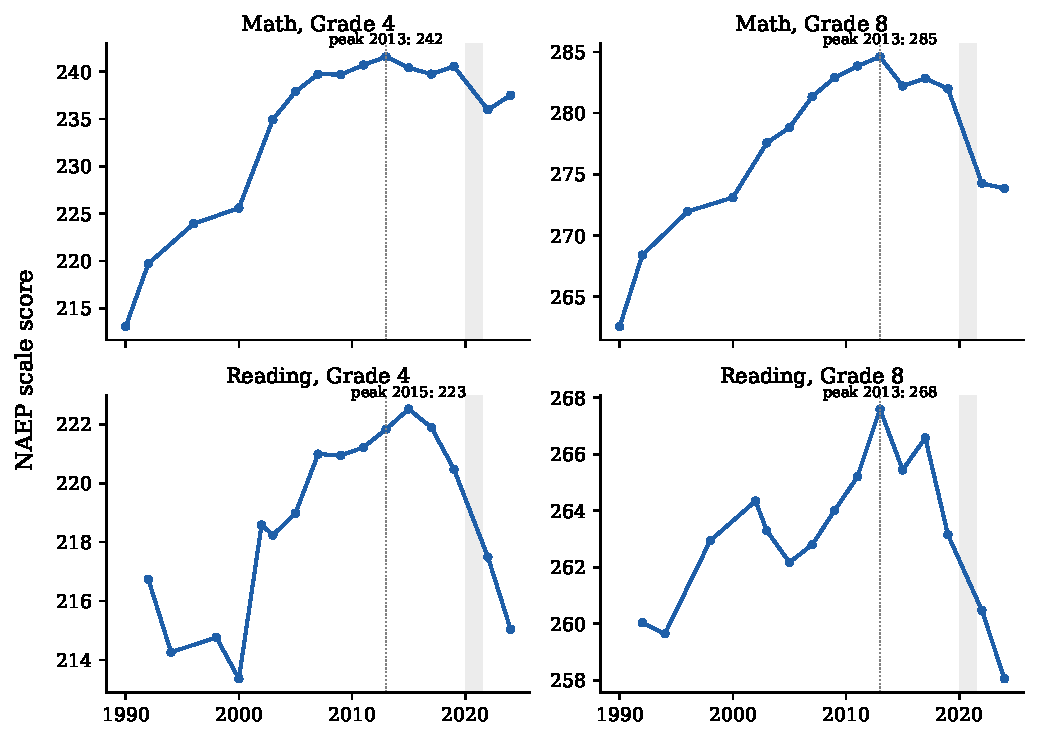
\includegraphics[width=.92\textwidth]{fig_national_trends.pdf}
\caption{National average NAEP scale scores, 1990--2024. All four series peak around 2013 and decline thereafter, with the sharpest drop in the pandemic window. The dotted line marks 2013; the shaded band marks pandemic-disrupted schooling. Data: NAEP Data Service API.}
\label{fig:national}
\end{figure}

\begin{table}[tbp]
\centering\small
\caption{National average score changes by period (NAEP scale points).}
\label{tab:changes}
\begin{tabular}{lccccc}
\toprule
 & \multicolumn{3}{c}{Change by period} & \multicolumn{2}{c}{Total 2013--2024} \\
\cmidrule(lr){2-4}\cmidrule(lr){5-6}
Series & 2013--19 & 2019--22 & 2022--24 & Points & SD units \\
\midrule
Mathematics, grade 4 & $-1.0$ & $-4.6$ & $+1.5$ & $-4.1$ & $-0.14$ \\
Mathematics, grade 8 & $-2.6$ & $-7.7$ & $-0.4$ & $-10.8$ & $-0.30$ \\
Reading, grade 4     & $-1.4$ & $-3.0$ & $-2.5$ & $-6.8$ & $-0.19$ \\
Reading, grade 8     & $-4.4$ & $-2.7$ & $-2.4$ & $-9.5$ & $-0.28$ \\
\bottomrule
\end{tabular}
\end{table}

Table~\ref{tab:changes} decomposes the decline. Three observations matter for everything that follows. First, the total losses are large: 0.14--0.30 student-level SD, roughly one grade level of learning in grade 8. In level terms, 2024 grade 4 mathematics matches 2005; grade 8 mathematics matches 2000; grade 4 reading is below every year since 1998; and grade 8 reading (258.0) is below its previous historical minimum. Second, the pandemic window accounts for the majority of the mathematics decline (71\% of the grade 8 total) but \emph{less than half} of the reading decline at grade 8, where 46\% of the loss had already occurred by 2019. Third, the post-pandemic period has produced essentially no aggregate recovery: only grade 4 mathematics regained ground (about a third of its pandemic loss), while both reading series fell \emph{further} between 2022 and 2024.

\subsection{The Long-Term Trend assessment: the same timing on unchanged content}
\label{sec:ltt}

The LTT data (Figure~\ref{fig:ltt}) rule out the possibility that the main-NAEP decline is an artifact of framework or administration changes. On test content held essentially constant since the 1970s, age 9 and age 13 scores peaked in 2012 and were already falling before the pandemic. Age 13 mathematics fell from 285 in 2012 to 280 in fall 2019, and age 13 reading from 263 to 260, \emph{before any school closed}. The pandemic then produced the largest drops ever recorded in the series. Age 9 mathematics fell 7 points between early 2020 and 2022 (its first statistically significant decline ever), and age 13 mathematics fell 9 further points by fall 2022, landing at its 1992 level. Age 13 reading in 2023 (256) was statistically indistinguishable from its 1971 baseline: a half-century of progress erased for the median young adolescent. The 2025 wave, released in June 2026, shows the post-pandemic period diverging by age. At age 9, students recovered 3.8 points in both subjects, putting reading within 1.3 points of its pre-pandemic level. At age 13, scores were flat (mathematics 270.3 against 270.7 in 2023; reading 256.1 against 255.7), leaving age-13 mathematics 14.7 points below its 2012 peak and age-13 reading still at its 1971 level.

\begin{figure}[tbp]
\centering
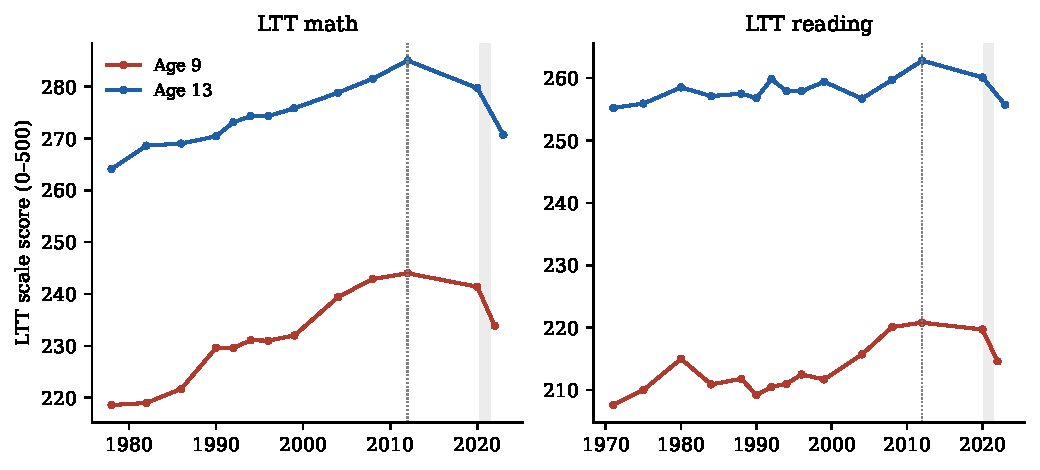
\includegraphics[width=.92\textwidth]{fig_ltt.pdf}
\caption{NAEP Long-Term Trend average scores, ages 9 and 13, 1971--2025. Both ages peak in 2012 and decline before the pandemic; the pandemic-era drops are the largest in the series. The age 9 ``2020'' point was assessed January--March 2020 (pre-pandemic) and the age 13 ``2020'' point in fall 2019; the 2025 points were assessed in the 2024--25 school year. The dotted line marks 2012. Data: NCES Digest tables 221.85/222.85, validated against the LTT Data Service; 2025 wave from the LTT Data Service (\texttt{evidence/ltt\_2025.md}).}
\label{fig:ltt}
\end{figure}

\subsection{The distributional signature: collapse at the bottom}
\label{sec:dist}

The most diagnostic fact in the data is \emph{where} in the achievement distribution the losses occurred. Figure~\ref{fig:pctile} plots score changes since 2013 at the 10th through 90th percentiles for grade 8; Figure~\ref{fig:lttpct} shows the same comparison for the LTT, split into pre-pandemic (2012$\rightarrow$2020), pandemic (2020$\rightarrow$2022/23), and post-pandemic (2022/23$\rightarrow$2025) windows.

\begin{figure}[tbp]
\centering
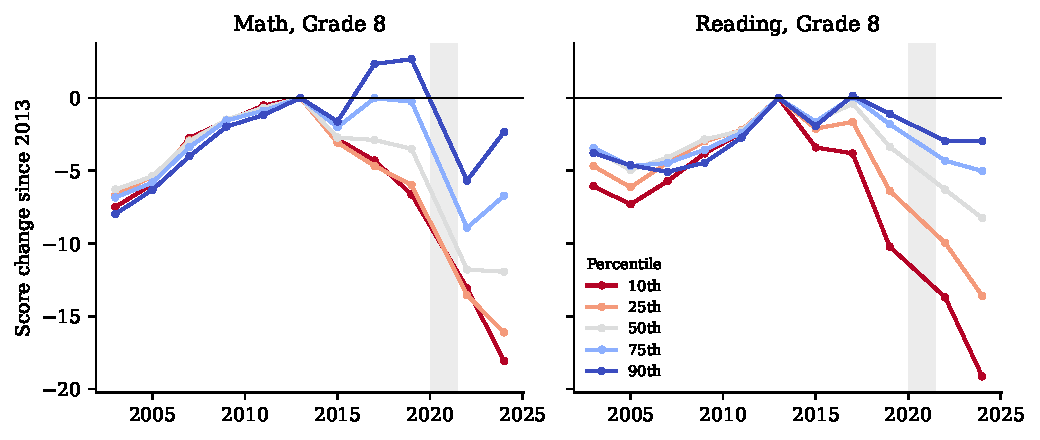
\includegraphics[width=.92\textwidth]{fig_percentiles_g8.pdf}
\caption{Grade 8 score changes since 2013 by percentile. Losses are deepest at the bottom of the distribution; before the pandemic the top held steady or improved. Data: NAEP Data Service API.}
\label{fig:pctile}
\end{figure}

\begin{figure}[tbp]
\centering
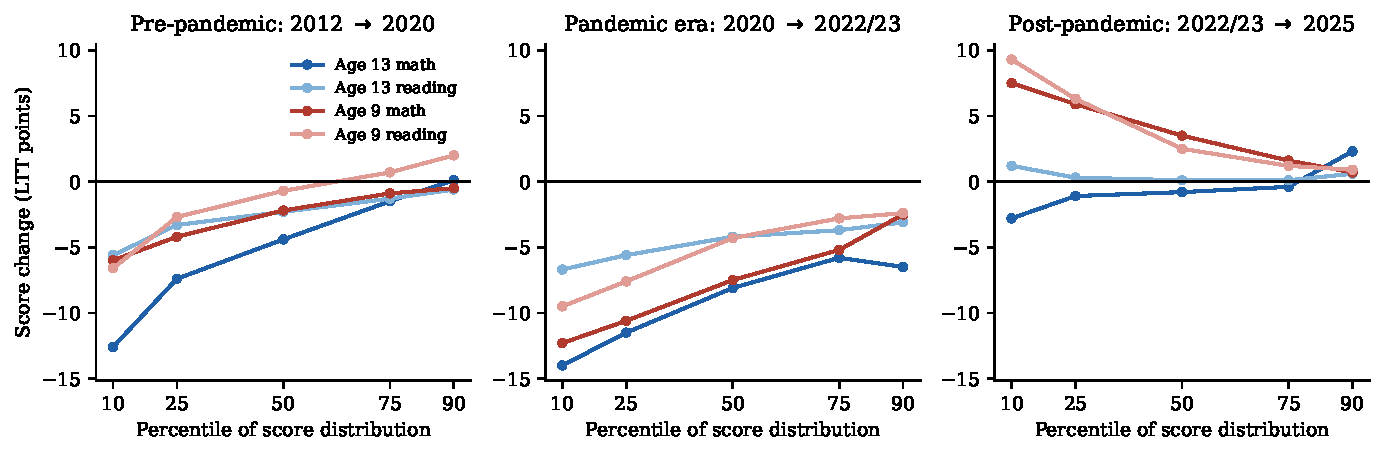
\includegraphics[width=.92\textwidth]{fig_ltt_percentiles.pdf}
\caption{LTT score changes by percentile in three windows: pre-pandemic (left), pandemic era (center), and post-pandemic (right). The pre-pandemic decline is concentrated almost entirely among low performers. The pandemic-era decline hits everywhere but is steepest at the bottom. After 2022/23 the recovery is bottom-led at age 9, while at age 13 the bottom of the mathematics distribution keeps falling as the top recovers. Data: LTT Data Service.}
\label{fig:lttpct}
\end{figure}

Before the pandemic, the decline was almost exclusively a bottom-of-the-distribution phenomenon. Between 2012 and 2020, age 13 LTT mathematics fell 12.6 points at the 10th percentile, 7.4 at the 25th, and 4.4 at the median, while \emph{rising} 0.1 points at the 90th. Main NAEP shows the same pattern: between 2013 and 2019, grade 8 mathematics fell 6.6 points at the 10th percentile while \emph{gaining} 2.7 points at the 90th, and grade 8 reading fell 10.2 points at the 10th percentile against 1.1 at the 90th. America's strongest students were holding steady or improving through 2019; its weakest students had been losing ground for years before anyone had heard of COVID-19.

The pandemic broke this pattern in an informative way: the 2019--2022 losses appear across the entire distribution. In grade 8 mathematics the drop was essentially uniform, 6--9 points at every percentile, consistent with a shock (school disruption) that hit all students rather than only struggling ones. After 2022, the top of the distribution began recovering while the bottom kept falling: in grade 4 mathematics, 2022--2024 changes ranged from $+2.7$ points at the 75th percentile to $-0.6$ at the 10th.

The 2025 LTT results (Figure~\ref{fig:lttpct}, right panel) extend this divergence and split it by age. At age 13 the fan-out continued: between the 2023 and 2025 assessments, mathematics fell a further 2.8 points at the 10th percentile while rising 2.3 points at the 90th. That pushed the age-13 mathematics 90--10 gap to 114 points, 25 points wider than in 2012 and the widest in the series' half-century history. At age 9, by contrast, the recovery is real and concentrated where the losses were: +7.5 points at the 10th percentile in mathematics and +9.3 in reading, against +0.7 and +0.9 at the 90th. The age-9 turnaround is the first bottom-led improvement anywhere in this report's data. It also post-dates the 2024 main-NAEP assessment, where the grade 4 bottom decile was still falling. The two are consistent if the youngest students' rebound began only in the 2024--25 school year, a reading the 2026 main NAEP will adjudicate.

The cumulative effect on inequality is unprecedented in NAEP's history. The 90--10 gap (Figure~\ref{fig:gap}) widened between 2013 and 2024 by 13 points in grade 4 mathematics (75$\rightarrow$89), 16 points in grade 8 mathematics (93$\rightarrow$109), 15 points in grade 4 reading, and 16 points in grade 8 reading. In every case the 2024 gap is the widest ever recorded.

\begin{figure}[tbp]
\centering
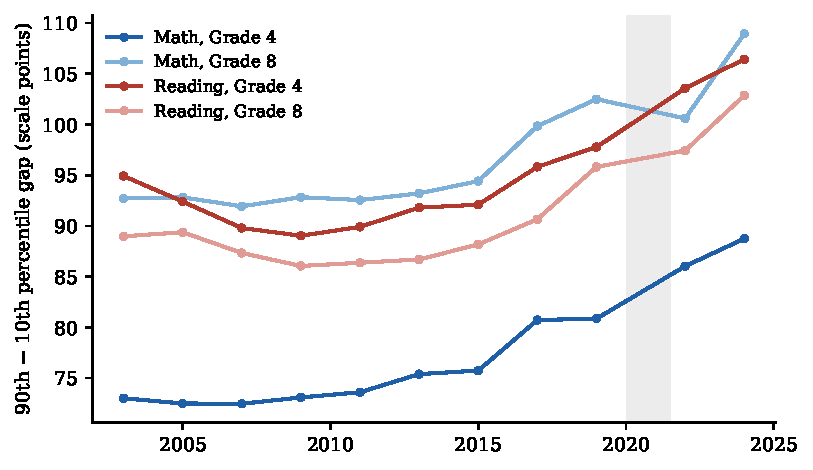
\includegraphics[width=.7\textwidth]{fig_gap9010.pdf}
\caption{Gap between the 90th and 10th percentile scores, 2003--2024. The gap widens after 2013 in every series; by 2024 each is the widest on record. Data: NAEP Data Service API.}
\label{fig:gap}
\end{figure}

\subsection{Subgroups: declines within every group}
\label{sec:subgroups}

Score declines appear \emph{within} essentially every demographic subgroup, which constrains compositional explanations (Section~\ref{sec:h5}). Between 2013 and 2024, grade 8 mathematics fell 8.3 points among White students, 11.4 among Black students, 13.1 among Hispanic students, and was about flat ($-1.1$) only among Asian/Pacific Islander students. Both NSLP-eligible (lower-income) and non-eligible students lost ground through 2022 (grade 8 mathematics: $-10.4$ and $-9.9$ respectively). Pre-pandemic, the within-group pattern mirrors the percentile pattern: between 2013 and 2019 grade 8 mathematics scores among lunch-eligible students fell 3.6 points while non-eligible students lost only 1.0; Asian/Pacific Islander students \emph{gained} 3.5 points. Figure~\ref{fig:lunch} shows the level trends by lunch eligibility.

\begin{figure}[tbp]
\centering
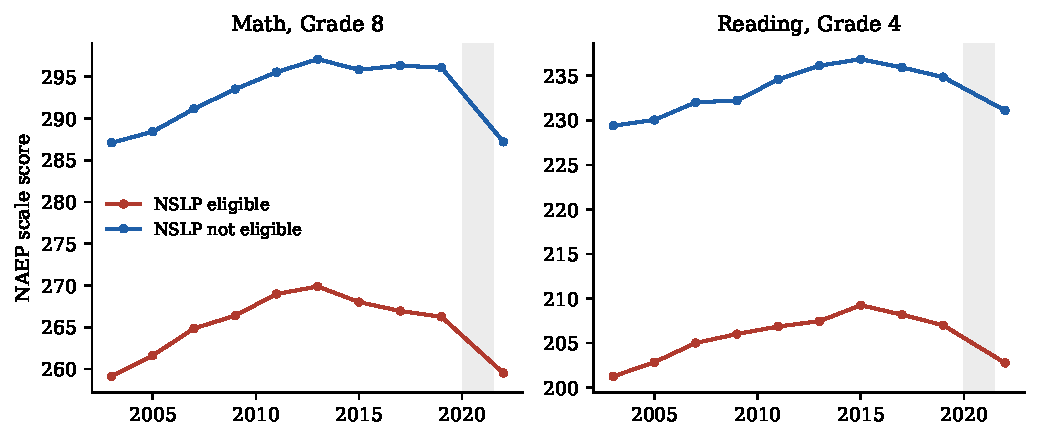
\includegraphics[width=.92\textwidth]{fig_lunch.pdf}
\caption{Average scores by National School Lunch Program eligibility (available through 2022). Both groups decline through 2022, with larger pre-pandemic losses among eligible (lower-income) students. Data: NAEP Data Service API.}
\label{fig:lunch}
\end{figure}

\subsection{Geography: a national phenomenon, modulated by pandemic policy}
\label{sec:states}

The decline is not regional. Between 2013 and 2019, 75--94\% of states (depending on series) posted declines; by 2024, between 88\% and 100\% of states remained below their 2013 level. No state escaped the national trend in grade 8 mathematics. Two partial exceptions are instructive. Mississippi rose from 49th to 29th in grade 4 reading between 2013 and 2019 following its 2013 early-literacy reform \citep{spencer2024}, and a handful of states (e.g., Alabama, Louisiana) regained or exceeded pre-pandemic grade 4 mathematics levels by 2024.

State variation \emph{within} the pandemic window lines up with schooling-mode differences (Section~\ref{sec:h1}). States' 2019--2022 drops in grade 4 mathematics ranged from about $-13$ points to roughly zero. The states that fell most recovered somewhat faster afterward (correlation between 2019--22 change and 2022--24 change $\approx -0.3$ to $-0.5$; Figure~\ref{fig:states}), consistent with partial mean reversion as in-person schooling resumed. But the rebound slopes are shallow (about $-0.4$): most of the pandemic-window loss has, so far, been persistent rather than transitory.

\begin{figure}[tbp]
\centering
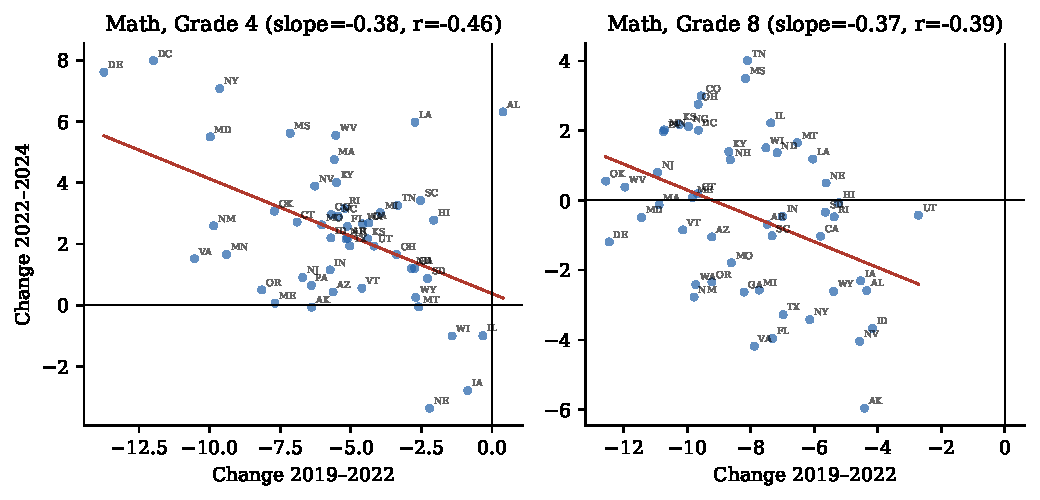
\includegraphics[width=.92\textwidth]{fig_states.pdf}
\caption{State-level pandemic losses versus post-pandemic recovery, mathematics. Each point is a state. States that lost the most during the pandemic window recovered somewhat faster afterward, but the rebound is shallow relative to the losses. Data: NAEP Data Service API.}
\label{fig:states}
\end{figure}

\subsection{International context: America is not alone}
\label{sec:intl}

The U.S. decline is part of a broader rich-world phenomenon (Figure~\ref{fig:intl}). The OECD-average PISA mathematics score fell 22 points between 2012 and 2022 (494$\rightarrow$472) and reading fell 20 points, declines that began \emph{before} the pandemic. The OECD itself concluded that the fall was ``only partly attributable to the COVID-19 pandemic,'' noting that reading and science had been sliding for roughly a decade \citep{oecd2023}. Twelve OECD systems, including Finland, the Netherlands, Belgium, and Canada, show statistically significant mathematics declines beginning before 2018. One U.S. series is an apparent exception: U.S. PISA \emph{reading} was flat (505$\rightarrow$504) between 2018 and 2022 while the OECD average fell 11 points, so the U.S. position relative to peers improved even as its NAEP reading scores fell. One reconciliation is that PISA samples 15-year-olds, whose NAEP-cohort losses were smaller than younger students'. U.S. TIMSS mathematics tells the same story as NAEP: grade 8 scores fell 27 points between 2019 and 2023, back to mid-1990s levels, with the lowest 10th-percentile scores since the study began \citep{nces2024timss}.

\begin{figure}[tbp]
\centering
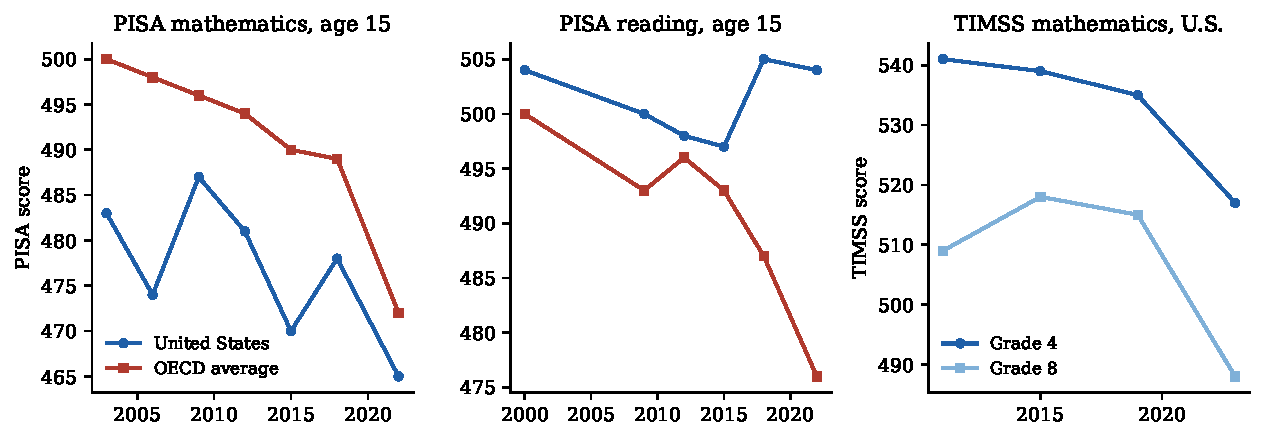
\includegraphics[width=.99\textwidth]{fig_intl.pdf}
\caption{International assessments: PISA mathematics and reading (U.S. vs.\ OECD average) and U.S. TIMSS mathematics. The OECD-average declines begin before the pandemic; U.S. TIMSS falls in step with NAEP. Data: NCES/OECD publications.}
\label{fig:intl}
\end{figure}

\subsection{Seniors and adults: the decline is not confined to grades 4 and 8}
\label{sec:adults}

Two further populations complete the picture, and both carry unusual inferential weight because the usual school-policy explanations apply to them weakly or not at all. Grade 12 NAEP (2024 results released in September 2025) shows the same pattern as the younger grades. Mathematics peaked in 2013 (153.5), drifted down through 2019 (150.3), and fell to its lowest level ever recorded in 2024 (146.9), with 2019--2024 losses of 5 points at the 10th percentile against no significant change at the 90th. Reading fell to its own record low (282.6); its 1992--2024 percentile changes ($-24$ at the 10th percentile, $-2$ at the 75th) are the three-decade version of the bottom-collapse \citep{nces2025g12}.\footnote{Grade 12 weighted student participation was 68\% in 2024, well below the grades 4/8 rates; G12 levels warrant more caution than the younger-grade series.}

The adult evidence is the more telling of the two. The 2023 PIAAC assessment of adults aged 16--65 \citep{ncespiaac2024,oecd2024adult} found U.S. literacy down 12 points from 2017 and numeracy down 6. The decline was concentrated almost entirely at the bottom: the share at or below Level~1 rose from 19\% to 28\% in literacy and from 29\% to 34\% in numeracy, while the share at Levels 4--5 was stable. The same happened across the OECD: literacy fell in 19 OECD countries between 2012 and 2023, with the bottom decile declining and the top decile improving in most. Adults are not subject to school accountability, the Common Core, school funding, teacher quality, or school absenteeism. A force that simultaneously lowers the floor of measured literacy and numeracy among 40-year-olds in nineteen countries and among 13-year-olds in American public \emph{and} Catholic schools is not plausibly an education-policy variable: nothing education policy does reaches all of those populations at once. \citet{malkus2025theories} flagged the adult parallel using earlier PIAAC rounds as one of his four keys; the 2023 cycle sharpens it.\footnote{NCES cautions that cross-cycle PIAAC comparisons involve assessment and scoring changes; the trend-comparable estimates show the same pattern with a smaller literacy decline (9 points).}

\subsection{Summary of facts to be explained}

The preceding subsections establish eight facts. Any successful explanation must account for: (F1) a peak in 2012--2013 and slow decline through 2019; (F2) pre-2019 losses concentrated overwhelmingly at the bottom of the distribution, with the top flat or rising; (F3) a large, across-the-distribution drop in 2019--2022; (F4) continued post-2022 decline in reading and at the bottom of the adolescent distributions, against recovery at the top and (first visible in the 2025 LTT) a bottom-led rebound among 9-year-olds; (F5) declines within every demographic group and nearly every state; (F6) similar pre-pandemic declines across many rich countries; (F7) record-high achievement inequality; and (F8) the same bottom-concentrated decline among high-school seniors and, in PIAAC, among adults across the OECD, populations to which most school-policy explanations do not apply.

\section{Candidate Explanations}\label{sec:candidates}

Eight candidate explanations recur in the research literature and in public debate. Each generates predictions specific enough to check against the facts of Section~\ref{sec:verify}. The eight are:

\begin{enumerate}
\item[H1.] \textbf{Pandemic disruption.} School closures, remote instruction, and associated social disruption caused learning loss.
\item[H2.] \textbf{Smartphones and digital media.} The post-2012 saturation of adolescent life by smartphones and social media displaced reading and homework and fragmented attention.
\item[H3.] \textbf{Accountability retreat.} The dismantling of No Child Left Behind's test-based accountability (waivers from 2012, ESSA from 2015) removed pressure that had propped up achievement among low performers.
\item[H4.] \textbf{Great Recession funding cuts.} State school-funding cuts after 2008 reduced school quality for the cohorts tested in the mid-2010s.
\item[H5.] \textbf{Demographic change.} A rising share of disadvantaged students mechanically lowered average scores.
\item[H6.] \textbf{Chronic absenteeism.} Students stopped attending school regularly after the pandemic.
\item[H7.] \textbf{Declining reading practice.} Children read less, for school and pleasure, eroding literacy skills.
\item[H8.] \textbf{Other: teacher shortages, the Common Core transition, lowered expectations/grade inflation, adolescent mental health.}
\end{enumerate}

Two notes bound this list. It is drawn from the explanations prominent in research and public debate and makes no claim to exhaust the possible causes; the elimination logic used below is only as strong as the candidate set itself. And it is not closed: candidates proposed by readers of earlier drafts (rising immigration, political polarization, school-discipline reform, and deteriorating adolescent mental health) are taken up in Section~\ref{sec:h8}, and further avenues examined and set aside are recorded in Section~\ref{sec:setaside}.

\section{Testing the Hypotheses}\label{sec:testing}

\subsection{H1: Pandemic disruption --- the 2019--2022 drop, dose-response evidence, and the recovery record}
\label{sec:h1}

\textbf{Predictions.} A sharp drop between the 2019 and 2022 assessments; larger losses where schooling was remote longer; recovery as schooling normalized; no effect before 2020.

\textbf{Evidence.} The 2019--2022 drop is unambiguous and its causal link to schooling disruption is among the best-documented findings in modern education research. Districts that were remote for more than half of 2020--21 saw mathematics achievement growth shortfalls of 0.44~SD in high-poverty schools, versus about 0.17~SD where instruction stayed in person \citep{goldhaber2023}. Across twelve states, district math pass rates fell 14.2 percentage points on average in spring 2021, but only 4.1 points in districts that remained fully in person \citep{jack2023}. The dose-response gradient, its replication across data sets, and the coincidence in time make H1 conclusively established for phase two, particularly for mathematics, which is learned mostly in school. Consistent with this, the 2019--2022 NAEP drop was nearly uniform across the achievement distribution (Section~\ref{sec:dist}), as expected from a shock to schooling itself.

Two equally important negative results bound the hypothesis. First, H1 predicts nothing before 2020, yet roughly a quarter to a half of the total 2013--2024 decline predates the pandemic (Table~\ref{tab:changes}), including the entire 2012--2020 collapse at the bottom of the LTT distribution. Second, H1 predicts recovery, and recovery has been feeble: by spring 2023 students had regained only about a third of pandemic mathematics losses and a quarter of reading losses \citep{kane2024}; by 2025 only 17\% of students were in districts at or above 2019 mathematics levels \citep{kane2025}; and NAEP reading fell \emph{further} after 2022. The 2025 LTT adds an age split that sharpens rather than relieves this: 9-year-olds have begun a genuine, bottom-led recovery, but 13-year-olds (the cohorts whose elementary schooling the pandemic interrupted) remained flat through the 2024--25 school year, with bottom-decile mathematics still falling five years after the shock. The $\sim$$-0.4$ slope in Figure~\ref{fig:states} says the same thing in the NAEP data: states recovered only a fraction of their own excess pandemic losses.

\textbf{Assessment.} \emph{Established by direct causal evidence as the dominant cause of phase two (roughly half to three-quarters of the mathematics decline, less of reading); cannot explain phase one; the failure to recover requires additional explanation (H6, and the bottom-distribution forces of H2/H3).}

\subsection{H2: Smartphones and digital media --- timing, breadth, and the ban literature}
\label{sec:h2}

\textbf{Predictions.} Decline beginning when smartphones saturated childhood ($\sim$2012--2015); present across countries, subjects, and demographic groups; strongest in reading and among students with the least adult structure; displacement of reading and homework time.

\textbf{Evidence on timing.} The exposure and the decline moved together. Teen smartphone ownership in the U.S. went from 23\% in 2011 to 37\% in 2012, 73\% by 2015, and 95\% by 2018, with 45\% of teens online ``almost constantly'' by 2018 \citep{pew2013,pew2018}. The achievement peak (2012--2013) coincides almost exactly with the takeoff. Adolescent entertainment screen time reached 7h22m/day by 2019 and 8h39m by 2021 \citep{commonsense2021}. Recreational reading collapsed on the same schedule, and mostly \emph{before} the pandemic: the share of 13-year-olds reading for fun almost daily fell from 27\% in 2012 to 17\% in 2020 and 14\% in 2023, where it stayed in 2025, while the share who never or hardly ever read rose from 22\% in 2012 to roughly 30\% in every assessment since 2020 (Figure~\ref{fig:fun}).

\textbf{Evidence on breadth.} H2 directly predicts fact F6, the synchronized pre-pandemic decline across rich countries with very different school policies, funding trends, and accountability regimes \citep{oecd2023}, and fact F8, its extension to adults, a breadth no school-policy candidate shares. The exposure is as broad as the outcome: within PISA 2022, 65\% of students across the OECD (66\% in the U.S.) reported digital-device distraction in mathematics class \citep{oecd2024}.

The PISA 2022 student microdata (613{,}744 students) allow those associations to be re-estimated with socioeconomic adjustment; estimates combine all ten plausible values by Rubin's rules, use final student weights, cluster by school, and adjust for a quadratic in the PISA socioeconomic index. Students reporting distraction in most or every mathematics lesson score 13.2 points lower in the U.S. (SE 3.9) and 15.0 points lower pooled across the OECD (SE 1.3) than less-distracted peers, and students reporting more than five hours of daily leisure device use at school score 40.5 points (SE 1.7) below light users. The OECD's published bivariate gaps survive socioeconomic adjustment essentially intact. These are associations, not causal estimates; the stronger support for H2 lies in the timing, the cross-national synchrony, the adult parallel, and the quasi-experimental ban literature below.

\textbf{Fit to the distributional signature.} The microdata also speak directly to where the exposure sits. Within countries, every device-engagement measure is monotonically concentrated at the bottom of the score distribution. Comparing students in their country's bottom vs.\ top mathematics quartile (OECD pooled, weighted): 32\% vs.\ 24\% report frequent classroom distraction, 8.2\% vs.\ 2.7\% report 5-plus hours of leisure device use at school, 24\% vs.\ 12\% report anxiety when their device is not nearby, and only 48\% vs.\ 71\% report turning off notifications in class.

The same measures are nearly \emph{flat across socioeconomic quartiles} (e.g., distraction 27.9\% in the lowest ESCS quartile vs.\ 25.8\% in the highest): heavy, poorly regulated device engagement is a low-\emph{performer} phenomenon, not a low-\emph{income} phenomenon. That matches the decline's signature, bottom-concentrated within every demographic group (Section~\ref{sec:subgroups}), in a way no compositional story does. Causality plausibly runs both ways (struggling students may retreat to screens), and the broader literature finds displacement harms students with the least self-regulation most \citep{haidt2024}; what the microdata establish is that the exposure profile and the damage profile coincide.

\textbf{Causal evidence from phone bans.} The hypothesis is no longer purely associational: a small quasi-experimental literature studies what happens when schools remove phones, and its effect pattern matches the decline's signature. Staggered school-level bans in four English cities raised test scores by 6.4\% of a standard deviation on average, and by \emph{14.2\% of a standard deviation for previously low-achieving students, with no effect on high achievers} \citep{belandmurphy2016}---the mirror image of the bottom-concentrated decline. Staggered Norwegian middle-school bans raised girls' GPA (+0.08 SD), cut bullying by $\sim$0.4 SD, and reduced psychological-symptom GP visits, with the largest gains for low-SES girls \citep{abrahamsson2024}. Spanish regional bans produced PISA gains worth more than half a year of learning \citep{beneito2022}. The first U.S. causal evidence, from Florida's 2023 ban, finds test-score gains emerging in the second year alongside reduced unexcused absences, linking the phone and attendance channels directly \citep{figlio2025}. The Swedish null \citep{kessel2020}, in a setting where teachers could already confiscate phones, indicates that the margin that matters is binding restrictions.

A far larger test is queued: the staggered state-level rollout of U.S. bans (one state in 2023--24, five by 2024--25, roughly twenty-five by 2025--26) against NAEP 2026, with the design and policy coding specified in this project's repository in advance of the data.

\textbf{Corroboration from an independent literature: fertility and family formation.} A new quasi-experimental literature aims the same shock at an entirely different outcome and arrives at the same structure. \citet{myershooper2026} exploit AT\&T's exclusive iPhone carrier deal (2007--2011), under which early smartphone access varied with pre-existing AT\&T coverage across counties: iPhone access reduced births by 4.5--8.0\% at ages 15--19 and 3.2--6.6\% at ages 20--24, with placebo tests on rival carriers' coverage returning nulls. In their estimates, smartphone diffusion accounts for a third to a half of the total fertility-rate decline, and the pathway evidence points to reduced in-person interaction. \citet{hudsonmoscoso2026} instrument county 4G rollout with terrain ruggedness and find teen births fell first and fastest where high-speed mobile arrived earliest, in the United States and, in a parallel design, England and Wales. The same instrument produces a rise in teen suicides, and time-diary data show teen in-person socializing roughly halving as digital leisure tripled.

Three features of these results matter here. The \emph{timing}: a break at 2007 compounding through the 2010--2015 4G wave, exactly the run-up to the 2013 achievement peak. The \emph{age profile}: effects decline monotonically in age and vanish for adults (in the authors' words, whatever the smartphone shock is doing, ``it is doing to teens''), the same adolescent-specific period effect that Section~\ref{sec:cohort} finds in achievement. And the \emph{identification}: rollout-based causal variation, not cross-sectional association. The age profile is, notably, the chief \emph{objection} to smartphones as an explanation of the adult-driven baby bust, and precisely the prediction the achievement hypothesis requires. The corroboration runs through the adolescent margin specifically: fixed-line broadband, a work tool for adults, if anything \emph{raised} fertility among educated women \citep{billari2019}.

Closest to the outcome studied here, \citet{jainstemper2024} link 3G arrival to 2.5 million PISA scores across 82 countries and estimate that mobile internet reduced mathematics, reading, and science scores by 0.04--0.08 standard deviations (about a quarter of a school year), concentrated among students with the least parental structure. Section~\ref{sec:fourg} runs the first within-U.S. version of this design and finds a precise null on the local arrival-timing margin. That null rejects the strong local form of the hypothesis, in which the harm rode on the cell-tower upgrade; the national, adoption-driven channel that the evidence above concerns is invisible to that design by construction.

\textbf{The age profile: a gradient, not a cliff.} The report's reliance on adolescent concentration may seem to sit awkwardly beside its use of the adult PIAAC decline as confirming evidence (Section~\ref{sec:adults}); the two are reconcilable, and the reconciliation is a prediction of the hypothesis rather than a patch to it. Exposure to the post-2012 digital environment is universal, but dose and developmental sensitivity are not: adolescents combine the heaviest and least-regulated use with the developmental window in which displaced reading, sleep, and attention compound into measured skill deficits. The hypothesis therefore predicts a gradient, not a cliff: effects largest among adolescents, present but weaker among adults. That is what the data show: the steepest collapse at age 13, record lows at grade 12, and a bottom-concentrated adult decline across nineteen OECD countries. The fertility literature's adult null is not a counterexample; it concerns births, not skills---PIAAC shows adult skills moved even where adult fertility did not. The 2025 LTT age split (9-year-olds recovering while 13-year-olds stagnate) fits the same gradient, since smartphone saturation at ages 11--14 far exceeds ages 5--9. The gradient is a commitment rather than an accommodation: adult losses outpacing adolescent losses, or an adolescent recovery arriving without any change in exposure, would count against the hypothesis.

\textbf{Exposure versus pathway.} ``Smartphones and digital media'' names an exposure, not a mechanism. If the exposure lowered achievement, it did so through one or more behavioral pathways, and the candidates differ: time displacement (screens crowd out reading, homework, and sleep); attention fragmentation (devices interrupt work in class and out of it); social displacement (less in-person interaction, the channel the fertility literature identifies); and degraded self-regulation (heavy use erodes the capacity to sustain effort). The evidence above speaks to each unevenly. The collapse of reading for fun (Figure~\ref{fig:fun}) is direct evidence of time displacement. The PISA distraction and notification items measure attention fragmentation. The time-diary shift from in-person socializing to digital leisure marks social displacement. And the ban studies' concentration of gains among previously low-achieving students reads most naturally as relief of distraction and weak self-regulation. This report establishes, at most, a reduced-form candidate: it does not adjudicate among these pathways. Its policy conclusions do not require that adjudication: the ban evidence and the attendance decompositions support binding school-day restrictions and attendance recovery whichever pathway dominates. The scientific account does require it, and that is where the empirical frontier sits.

\textbf{Assessment.} \emph{The leading candidate for phase one (and for the continued post-2022 slide in reading), on four lines of support: timing, international synchrony, quasi-experimental ban studies whose effect heterogeneity (low performers gain most when phones are removed) matches the distributional signature of the decline, and an independent rollout-based causal literature that recovers the same adolescent-concentrated, 2007-onset shock in fertility, mental health, and international test scores. The discriminating tests of Section~\ref{sec:sharper} consistently favor it over the school-policy alternatives, while this project's own adversarial test (Section~\ref{sec:fourg}) finds no detectable effect on the local arrival-timing margin. This is a consistency ranking, not a causal estimate; the pre-registered state phone-ban test against NAEP 2026 is the next direct test.}

\begin{figure}[tbp]
\centering
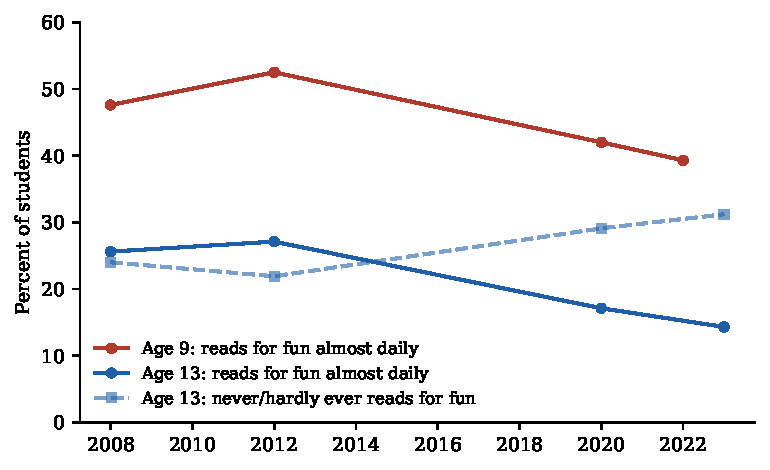
\includegraphics[width=.62\textwidth]{fig_readingfun.pdf}
\caption{Share of students reading for fun, NAEP LTT student survey. The decline pre-dates the pandemic. Data: LTT Data Service (variable S003501).}
\label{fig:fun}
\end{figure}

\subsection{H3: Accountability retreat --- timing, the distributional prediction, and two direct tests}
\label{sec:h3}

\textbf{Predictions.} Decline beginning after 2011--2012 (NCLB waivers) and deepening after 2015 (ESSA); concentrated among exactly the students accountability targeted---low performers and disadvantaged subgroups; U.S.-specific.

\textbf{Evidence.} The timing matches precisely: the first waivers releasing states from NCLB's consequences were granted in February 2012, covering 34 jurisdictions within a year; the Every Student Succeeds Act (December 2015) made the rollback permanent. The best causal evidence on NCLB found it had raised grade 4 mathematics by roughly 0.23~SD, with gains \emph{concentrated among low-achieving, Black, Hispanic, and lunch-eligible students}, and no effect on grade 4 reading \citep{deejacob2011}. The post-2012 decline is nearly a mirror image of those gains: largest at the 10th percentile, among disadvantaged groups, and (initially) clearer in mathematics at the grades accountability touched most. If a policy raised the floor, removing it should drop the floor, and the floor is what dropped (F2). Commentators including Chad Aldeman and former IES director Mark Schneider have pressed this reading of the NAEP record \citep{aldeman2025}.

The hypothesis has two limits and one point in its favor. It cannot explain F6 (Finland and the Netherlands did not pass ESSA), so it cannot be the sole driver. Because accountability operated through schools, it also predicts little about the collapse in out-of-school reading (Figure~\ref{fig:fun}). The point in H3's favor is Mississippi: the one state that \emph{intensified} early-grade stakes and instructional oversight after 2013 moved sharply against the national trend, with quasi-experimental evidence supporting a genuine policy effect \citep{spencer2024}.

\textbf{Assessment.} \emph{On the evidence of this section alone: supported as a contributor to the U.S. phase-one decline, especially its bottom-concentration; insufficient as a sole cause because the decline is international. Section~\ref{sec:sharper} subjects the hypothesis to two direct tests---sector comparison and waiver timing---and both come back unfavorable, leaving mainly its weaker national-climate form in play.}

\subsection{H4: Great Recession funding cuts --- timing, magnitudes, and the spending recovery}

\textbf{Predictions.} Declines among cohorts schooled during 2009--2015 austerity, reversing as spending recovered after 2013.

\textbf{Evidence.} The cuts were real and they did harm achievement; the magnitudes are simply far too small. Real per-pupil spending bottomed in 2012--13, 29 states cut per-pupil funding between 2008 and 2016 \citep{leachman2017}, and recession-induced cuts reduced achievement \citep{jacksonwigger2021}. The consensus causal estimate is roughly 0.03~SD per \$1,000 per pupil sustained for four years \citep{jacksonmackevicius2024}, so recession-era cuts on the order of \$1,000--\$1,500 per pupil could account for perhaps 0.03--0.05~SD, a fraction of the 0.14--0.30~SD decline. Spending also recovered steadily after 2013 while scores kept falling, the opposite of the predicted reversal. Funding cannot explain F2's top-stability (cuts hit whole districts), F6, or the post-2020 dynamics, when an unprecedented \$190 billion federal infusion accompanied historic losses (its measured effect, $\sim$0.008~SD per \$1,000 per student, was positive but small relative to the shock).

\textbf{Assessment.} \emph{Rejected as a major cause on magnitude and timing; plausibly a minor contributor to mid-2010s losses in the states that cut deepest.}

\subsection{H5: Demographic change --- within-group trends and a composition bound}
\label{sec:h5}

\textbf{Predictions.} Stable or rising scores within each subgroup, with composition shifts toward lower-scoring groups driving the aggregate down.

\textbf{Evidence.} The within-group facts in Section~\ref{sec:subgroups} directly contradict the prediction: scores fell within every major racial/ethnic group, within both lunch-eligibility groups, and for both sexes. Composition shifts were also too slow (Hispanic share up five percentage points over the decade; English learners up about one) to move national means more than a point or two, and the direction of some shifts (record-low child poverty in 2021) runs opposite the score trend. A back-of-envelope reweighting of 2024 grade 8 mathematics subgroup means at 2013 race shares recovers less than 2 of the 10.8 lost points.

\textbf{Assessment.} \emph{Rejected as an explanation of the decline (a 1--2 point compositional drag at most); within-group declines are the phenomenon itself.}

\subsection{H6: Chronic absenteeism --- timing, persistence, and the recovery stall}

\textbf{Predictions.} Score declines tracking the rise in absenteeism; weakest recovery where absenteeism stays elevated; no role before 2020.

\textbf{Evidence.} The administrative record places absenteeism in phase two, not phase one. Chronic absenteeism was flat at roughly 15\% from 2015 to 2019, so it cannot explain phase one; it then nearly doubled to about 28.5\% in 2021--22 and had retreated only to 23.5\% by 2023--24 \citep{malkus2025}. The persistence of elevated absence is exactly what F4 (no aggregate recovery) needs. The Council of Economic Advisers calculated that elevated absence could account for roughly 27\% of the 2019--2022 grade 4 mathematics decline and 45\% of the reading decline \citep{cea2023}, and \citet{dee2024} and the Education Recovery Scorecard identify it as a first-order obstacle to recovery. Absence is concentrated among low-income students, fitting the post-2022 divergence between the recovering top and the still-falling bottom.

\textbf{Assessment.} \emph{Strongly supported as a major amplifier of phase two and the leading proximate explanation for the failure to recover; explains little of phase one, though NAEP's own attendance item (Section~\ref{sec:attendance}) shows disengagement beginning to rise by 2017--2019, earlier than administrative data indicate. Absenteeism is partly a mediator: disengagement itself has causes (H1's disruption of attendance norms, H2's pull of screens).}

\subsection{H7: Declining reading practice --- H2's displacement pathway, measured directly}

The collapse in voluntary reading (Figure~\ref{fig:fun}) is among the largest behavioral shifts measured in any NAEP survey: daily reading for fun at age 13 halved between 2012 and 2023 and sat at that floor in 2025, with most of the fall pre-pandemic. Reading achievement requires volume of practice, and the grade 8 reading series, where losses began earliest (F1) and 46\% of the decline predates COVID, is where practice effects should show first. Classified properly, declining reading practice is therefore not a rival explanation but the time-displacement pathway of H2 (Section~\ref{sec:h2}), measured directly: the proximate cause is less reading; the open question is what replaced the reading and why. \emph{Assessment: the behavioral collapse is verified directly and matches the timing of the reading decline; it names a pathway rather than a root cause, and the root cause is what the remaining hypotheses contest.}

\subsection{H8: Other candidates}\label{sec:h8}

Readers of an earlier draft pressed four candidates on this report: rising immigration, increasing political polarization, school-discipline reform, and deteriorating adolescent mental health---the last of which the report had treated only as an outcome of the device shock, not as a rival cause of the decline. The first three can be handled briefly. Rising immigration is a compositional story and fails the same arithmetic as H5: scores fell within every demographic group, reweighting bounds the compositional contribution at 1--2 points (Section~\ref{sec:h5}), and the decline appears in Catholic schools, across rich countries, and among adults. Political polarization names a real change in American life but supplies no articulated pathway to a decline that is bottom-concentrated, adolescent-concentrated, internationally synchronized, and present among adults; its intensity is also distinctly American, while the decline is not. School-discipline reform has the right timing and a bottom-concentrated prediction but no clean policy variation independent of the variables already examined; Section~\ref{sec:setaside} records it as untested rather than rejected. Adolescent mental health cannot be dispatched; it is taken up at the end of this section.

\textbf{Teacher shortages and quality.} Vacancies and underqualified staffing are real ($\geq$36{,}000 vacant positions and $\geq$163{,}000 filled by underqualified teachers \citep{nguyen2024}), but they became acute mainly after 2020 and are concentrated in special education, STEM, and high-poverty schools; teacher-preparation enrollment fell through the 2010s. Plausibly a modest contributor to phase two and to bottom-distribution stagnation; the timing fits phase one poorly. \emph{Assessment: at most a minor contributor.}

\textbf{Common Core transition.} The standards' implementation (2014--15 in most states) coincides with the decline's onset, making them a recurring suspect, particularly in mathematics. The hypothesis has usable state variation: four states never adopted, three repealed in 2014, and Minnesota adopted only the reading standards. Section~\ref{sec:commoncore} tests it directly and finds that, pooled across grades and subjects, never-adopter states declined just as much (and more at grade 8). \emph{Assessment: rejected as a major cause by its own state-variation test.}

\textbf{Lowered expectations and grade inflation.} High-school GPAs rose from 3.17 (2010) to 3.36 (2021) while ACT scores fell \citep{act2022}, and course rigor and homework time show parallel softening. This evidence indicates that \emph{signals} of learning became disconnected from learning, masking the decline from parents and muting corrective pressure: an enabling condition more than a first cause. \emph{Assessment: contributing background condition; direction of causality unclear.}

\textbf{Adolescent mental health.} The strongest reader-proposed candidate warrants a fuller assessment. Adolescent mental health deteriorated on nearly the same schedule as achievement. The share of high-school students reporting persistent sadness or hopelessness rose from 28\% in 2011 to 37\% in 2019 (before the pandemic) and 42\% in 2021 \citep{cdcyrbs2023}, retreating only to 40\% in 2023 \citep{cdcyrbs2024}; the twelve-month prevalence of major depressive episodes among adolescents rose from 8.7\% in 2005 to 11.3\% in 2014 (stable through 2011, rising thereafter), an increase concentrated at ages 12--20 \citep{mojtabai2016}. This candidate passes the screens that eliminate the school-policy hypotheses (right timing, international reach \citep{haidt2024}, adolescent concentration) and, in its adolescent form, clears both bars of the dual-criterion test in Section~\ref{sec:synthesis}. Its fit is imperfect in two places: the distress rise is steepest among girls, a concentration with no counterpart in the achievement data; and it supplies no articulated channel to the adult skill decline (Section~\ref{sec:adults}), which the exposure account reaches through universal device use. But no test in this report eliminates it, and this report's data cannot separate it from H2: the rollout designs that link smartphone arrival to teen fertility also link it to worse adolescent mental health \citep{hudsonmoscoso2026}, and the Norwegian ban study finds that removing phones improves mental health and achievement together \citep{abrahamsson2024}. Distress may be a pathway from devices to disengagement, a joint product of the same shock, or an independent force for which devices are a covariate; the evidence assembled here cannot say which. \emph{Assessment: right timing, international, adolescent-concentrated; the strongest unresolved rival to the digital-media hypothesis, and not separable from it with this report's data.}

\subsection{Avenues examined and set aside}
\label{sec:setaside}

Several further hypotheses were tested or scoped and judged not to merit headline treatment; they are recorded here so the reader knows they were not overlooked.
\begin{itemize}
\item \emph{Opioid epidemic / family distress.} Regressing states' 2013--2019 bottom-decile changes on the change in CDC age-adjusted drug-overdose death rates yields right-signed but statistically null estimates in three of four series (the largest, grade 4 reading, has $r=-0.32$, $p=0.12$). With heavy geographic confounding and no dose-response consistency, the test neither supports nor rules out a contributing role.
\item \emph{School discipline reform.} The 2014 federal guidance and the accompanying decline in suspensions have the right timing and a bottom-concentrated prediction, but there is no clean cross-state policy variation independent of the accountability and political variables already examined. The hypothesis remains untested rather than rejected.
\item \emph{Cross-country smartphone-adoption timing vs.\ PISA declines.} Country-level adoption series are too inconsistently measured across sources to support a credible event-time alignment; this remains the right design for future work with better data.
\item \emph{Cannabis legalization.} This fails on first inspection: adolescent use was roughly flat through the 2010s in national surveys, and legalization timing is collinear with state politics and pandemic schooling mode.
\item \emph{PISA smartphone-use frequency.} The ICT item available for U.S. students was examined and discarded as an exposure measure: ``uses a smartphone several times daily'' is positively associated with scores (+70 points vs.\ never-users, SES-adjusted) because, in a 95\%-saturated population, the abstainers are a highly atypical, disadvantaged group. Frequency of use measures access, not excess; the hours-of-use and distraction items of Section~\ref{sec:h2} do not share this defect.
\end{itemize}

\section{Sharper Tests: Cohorts, Sectors, and Policy and Rollout Variation}
\label{sec:sharper}

The assessments above lean on timing and incidence. This section reports five sharper tests, each exploiting a dimension of the data that the candidate explanations treat differently: a cohort-matched decomposition separating period effects from cohort effects, a sector comparison against Catholic schools that federal accountability never governed, and three timing designs built from policy and rollout variation (release from NCLB, Common Core adoption, and the arrival of high-speed mobile internet). The standard is symmetric by design: each of the two leading phase-one hypotheses (H2 digital media, H3 accountability) faces a timing test built from its own variation and reported the same way, stating the margin the design identifies, the result with its minimum detectable effect, the form of the hypothesis the null rejects, and the channel that survives by construction. The waiver event study is the direct policy-variation test of H3; the quasi-experimental ban literature and the pre-registered state-ban test against NAEP 2026 (Section~\ref{sec:h2}) are the corresponding policy tests of H2; and the 4G-rollout event study is this project's own adversarial test of its leading candidate.

\subsection{Cohort vs.\ period: the losses accrue during adolescence}
\label{sec:cohort}

If successive birth cohorts were arriving at school weaker---because of early-childhood environment, poverty, or school quality in the early grades---declines should appear at grade 4 first and follow cohorts upward. If instead something in the post-2012 environment harms whoever is an adolescent at the time, grade 8 should fall regardless of how cohorts looked at grade 4. The data can separate these because the same birth cohort is observed at grade 4 and, four years later, at grade 8.

Define cohort-matched pseudo-growth as the grade 8 average in year $t$ minus the grade 4 average in year $t-4$. Figure~\ref{fig:cohort} (left) shows this quantity fell sharply for cohorts reaching grade 8 after 2013: mathematics pseudo-growth dropped from 44--46 points (2007--2013 cohorts) to about 41.5 points (2015--2019), and reading from 44--47 to 40.6 by 2019. Decomposing the 2013--2019 grade 8 decline: in mathematics, $-2.6 = +0.7$ (higher grade 4 entry scores of the later cohorts) $-3.3$ (less growth between grades 4 and 8); in reading, $-4.4 = +1.6 - 6.0$. \emph{The cohorts that drove the pre-pandemic grade 8 decline arrived at grade 4 at record levels and then lost ground during the middle-school years.} The right panel shows the same fact by birth year: the identical cohorts that look healthy in the age-9/grade-4 series collapse in the age-13/grade-8 series once their adolescence falls after roughly 2012.

This is a period effect concentrated in adolescence, not a cohort effect. It is unfavorable to explanations rooted in early childhood or school inputs broadly (which would depress grade 4 entry too), and it matches the exposure profile of smartphones and social media, which saturate ages 11--14 far more than ages 5--9. It is compatible with the accountability hypothesis only in the version where pressure mattered most in the middle grades. The result formalizes what \citet{petrilli2020} observed informally for two graduating classes and supplies the demonstration behind \citet{malkus2025theories}'s narrative argument against cohort-cascade accounts.

\begin{figure}[tbp]
\centering
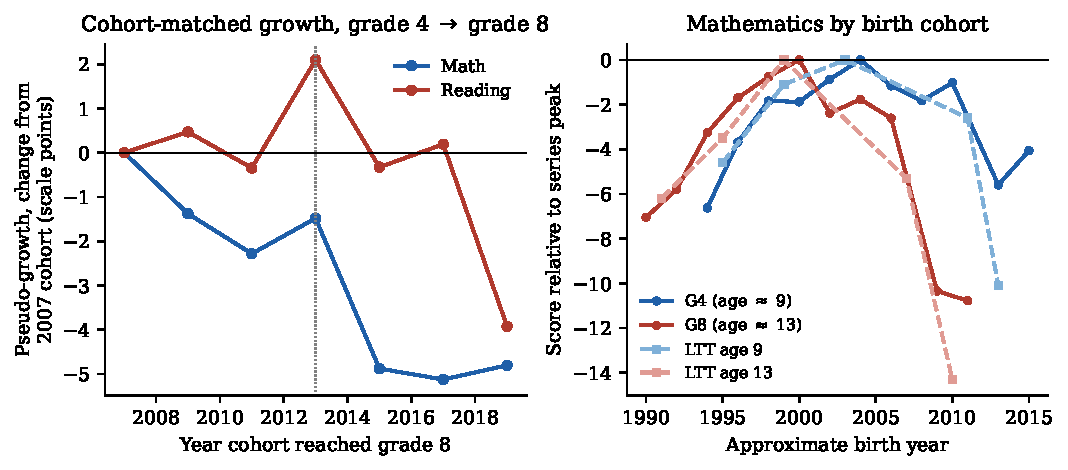
\includegraphics[width=.95\textwidth]{fig_cohort.pdf}
\caption{Cohort vs.\ period. Left: cohort-matched pseudo-growth (grade 8 mean minus the same cohort's grade 4 mean four years earlier), relative to the 2007 value. Right: mathematics scores by approximate birth year for four age groups, each relative to its series peak. Data: NAEP Data Service API; LTT.}
\label{fig:cohort}
\end{figure}

\subsection{Public vs.\ Catholic schools: an untreated-sector test}
\label{sec:sector}

Federal test-based accountability never applied to private schools, while smartphones and digital media saturated adolescent life in both sectors, so the two leading phase-one hypotheses make different predictions about private-school trends. \citet{malkus2015} sketched this test informally after a single cycle; this section runs it over the full window. NAEP reports Catholic-school results in every assessment year (overall private results are suppressed in several recent years for participation reasons), giving a usable untreated sector.\footnote{Catholic-school samples are far smaller than public ones, so their estimates are noisier, and Catholic enrollment is selected; level differences are uninformative. The comparison of \emph{trends} is the test.}

Reading provides the statistically informative sector contrast. Figure~\ref{fig:pubcath} shows changes since 2013; because Catholic estimates carry standard errors near 1.6 points (vs.\ 0.3 for public; Digest table 222.32a), formal tests matter here. Catholic grade 8 reading fell $-7.8$ points between 2013 and 2019 ($z=-3.4$ on published SEs), at least as much as the public-school decline of $-4.0$. The subject in which the pre-pandemic decline was largest and earliest was therefore falling just as fast inside schools that NCLB and its repeal never touched. A pure accountability story predicts flat private-sector trends; the reading evidence contradicts that prediction. In mathematics the Catholic samples are too noisy to be informative: the $-1.5$ change is indistinguishable from zero and from the public $-2.6$. Grade 4, where Catholic scores held flat while the public bottom decile fell, leaves room for an accountability contribution in the early grades. After 2019 the sectors diverge sharply and significantly in grade 8 mathematics: public schools fell 7.9 points more than Catholic schools ($z=-2.6$, using a conservative 2.5-point SE for recent Catholic estimates), leaving Catholic students by 2024 within 2.3 points of their 2013 level while public students were 11.4 points below. That divergence is consistent with private schools' shorter closures and lower post-pandemic absenteeism.

\begin{figure}[tbp]
\centering
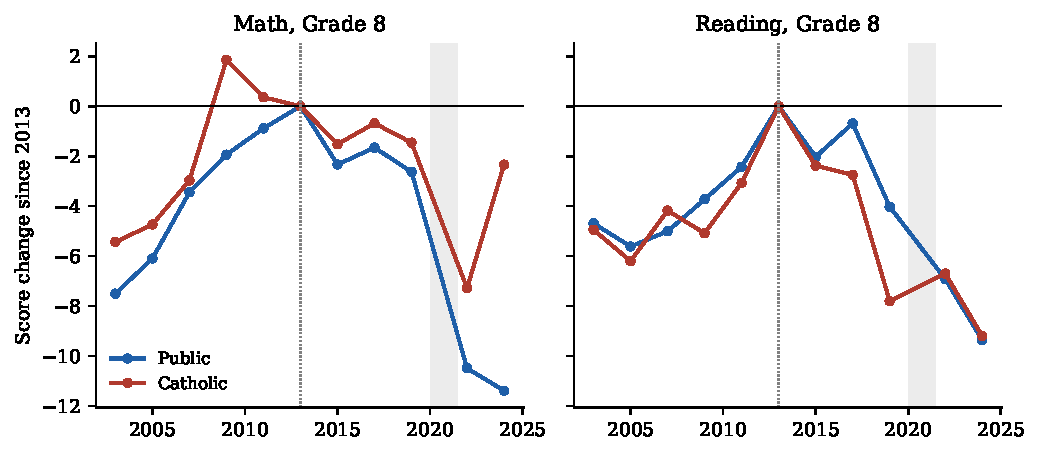
\includegraphics[width=.92\textwidth]{fig_pubcath.pdf}
\caption{Average scores by school sector, relative to 2013. Data: NAEP Data Service API (SCHTYPE), national.}
\label{fig:pubcath}
\end{figure}

\subsection{NCLB waiver timing: no detectable effect on the release-timing margin}
\label{sec:waiver}

If dismantling test-based accountability drove the decline, the dismantling itself supplies a test: states were released from NCLB's consequences at different times, and bottom-decile scores should have begun falling where and when the pressure came off. \citet{dewey2026} observe descriptively that post-2013 declines look similar in waiver and non-waiver states and note that the sustained-accountability counterfactual ``has never been tested''; this section provides the test. States received ESEA flexibility waivers in waves: eleven in early 2012, twenty-three more (plus DC) later in 2012, and eight in 2013--2014. Seven states (CA, IA, MT, NE, ND, VT, WY) never received one and remained formally under NCLB until ESSA took effect in 2017--18.\footnote{Approval dates compiled from the Department of Education's per-state ESEA flexibility pages, CRS Report R42328, and EdWeek's state-by-state tracking. Washington's waiver was revoked in April 2014; it is dropped from the panel after 2013.} The design identifies one margin: whether a state's formal release from NCLB consequences moved its scores, relative to states not yet or never released. It is the direct policy-variation test the accountability hypothesis invites.

The result is a null on the release-timing margin (Figure~\ref{fig:waiver}, using the state-percentile panel, 2003--2019, ending before the pandemic). Left panel: 10th-percentile grade 8 mathematics scores in early-waiver, late-waiver, and never-waiver states move essentially in lockstep; never-waiver states' bottom decile fell as much as waiver states' after 2012. Right panel: an event-study regression (early-waiver vs.\ never-waiver states, all four grade--subject cells pooled in within-cell SD units, state and year fixed effects, clustered by state) finds post-2012 coefficients near zero. A two-way fixed-effects estimate of the post-waiver effect on 10th-percentile scores is $+0.09$ SD with $p=0.50$ pooled, and is small and insignificant in every cell separately; effects at the 25th and 90th percentiles are likewise null. The one prior quasi-experimental estimate, \citet{bleiberg2020}'s binary waiver difference-in-differences on mean student-level NAEP scores through 2013, also found no average effect; the percentile results here extend that null to the part of the distribution where the decline actually occurred and through 2019.

Because the comparison group is only seven states, conventional cluster asymptotics are unreliable, so inference is re-done by randomization: permuting the waiver-timing assignment across states 2{,}000 times yields $p=0.46$ for the pooled estimate ($p=0.86$ for grade 8 mathematics in points). The test is informative, not merely underpowered. The randomization distribution implies an 80\%-power minimum detectable effect of about \emph{3.2 points} on grade 8 mathematics 10th-percentile scores (0.35 SD pooled across cells), less than half the $\sim$7-point gain \citet{deejacob2011} attribute to NCLB's adoption, which was concentrated among exactly these students. If withdrawing accountability had undone even half of what imposing it achieved, this design would very likely have detected it. One caveat: a joint test of pre-2011 event-study coefficients gives $p=0.08$, and early-waiver states were converging upward toward never-waiver states before treatment (visible in Figure~\ref{fig:waiver}). The pre-trend cuts both ways but does not rescue the hypothesis, since the post-2012 point estimates are wrong-signed for H3.

What the null rejects is the strong local form of the hypothesis, in which the formal release from NCLB consequences drove a state's low performers downward. What survives by construction is the national form: if the operative change was a nationwide shift in expectations and stakes, culminating in ESSA, it hit all states in the same years, is absorbed by the year fixed effects, and is invisible to this design. A waiver is one notch of deregulation, and this test prices only that notch. Whatever the accountability retreat did to American students' learning, it did not travel through the timing of a state's own release. Section~\ref{sec:fourg} holds this report's leading candidate to the same standard.

\begin{figure}[tbp]
\centering
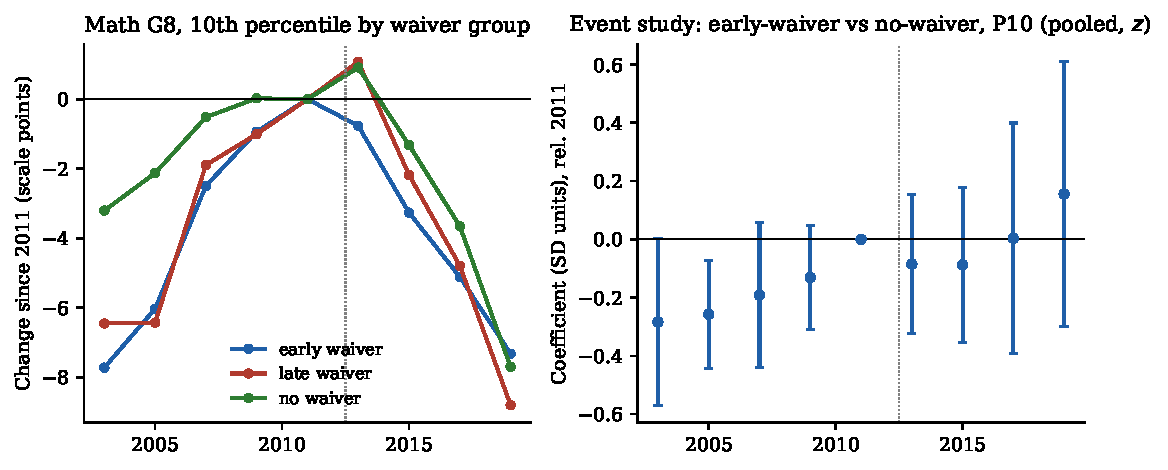
\includegraphics[width=.95\textwidth]{fig_waiver.pdf}
\caption{Waiver-timing tests, pre-COVID panel (2003--2019). Left: mean 10th-percentile grade 8 mathematics score by waiver group, relative to 2011. Right: event-study coefficients (early-waiver $\times$ year, base 2011, never-waiver comparison), all four grade--subject cells pooled in SD units; bars are 95\% confidence intervals, clustered by state. Data: NAEP Data Service API; waiver dates from ED/CRS/EdWeek.}
\label{fig:waiver}
\end{figure}

\subsection{Common Core: states that never adopted it declined anyway}
\label{sec:commoncore}

The Common Core is a further policy hypothesis with usable state variation. Nearly all states adopted the standards in 2010--2011 and implemented aligned assessments around 2014--15, exactly when scores began falling; critics have blamed the transition, particularly in mathematics, for the decline. Four states never adopted the standards (Alaska, Nebraska, Texas, Virginia), Minnesota adopted them in English language arts only, and three states formally repealed them in 2014 (Indiana, Oklahoma, South Carolina).\footnote{Adoption and repeal dates from NCES State Education Reforms Table 2.17, cross-checked against contemporaneous coverage. Post-2015 ``rebrands'' that retained aligned content (Georgia, New Jersey, Arizona, and others) are coded as adopters.}

The test fails to implicate the standards (Figure~\ref{fig:cc}). Between 2013 and 2019, never-adopter states' 10th-percentile scores fell less than adopters' in grade 4 mathematics, about as much in grade 4 reading, and \emph{more} than adopters' at grade 8 (mathematics: $-9.1$ vs.\ $-7.3$; reading: $-12.9$ vs.\ $-9.9$); pooled across the four series, the never-adopter difference in bottom-decile change is $-0.4$ points ($p=0.72$). The 2014 repealers look marginally better than adopters, but with three states the difference is uninformative. Minnesota offers a within-state subject contrast: its mathematics standards were never Common Core while its reading standards were. If the standards harmed mathematics, Minnesota's spared mathematics should have outperformed other states' treated mathematics; instead it fell slightly more ($-0.9$ points at grade 8 and $-2.9$ at grade 4, relative to other states), so avoiding the standards conferred no visible protection. (A mathematics-minus-reading triple-difference is $+2.3$ points at grade 8, the sign harm-to-mathematics would predict, but it is driven by Minnesota's unusually large relative reading decline of $-3.2$ points rather than by any mathematics outperformance, so it carries no evidence of harm to the treated subject; an earlier version of this report misread that statistic's direction.) A single state cannot carry much weight either way. As with the waiver test, the spillover caveat applies: never-adopter states still bought nationally aligned textbooks and materials. What the test rules out is the strong claim that adopting or keeping the standards is what drove a state's decline.

\begin{figure}[tbp]
\centering
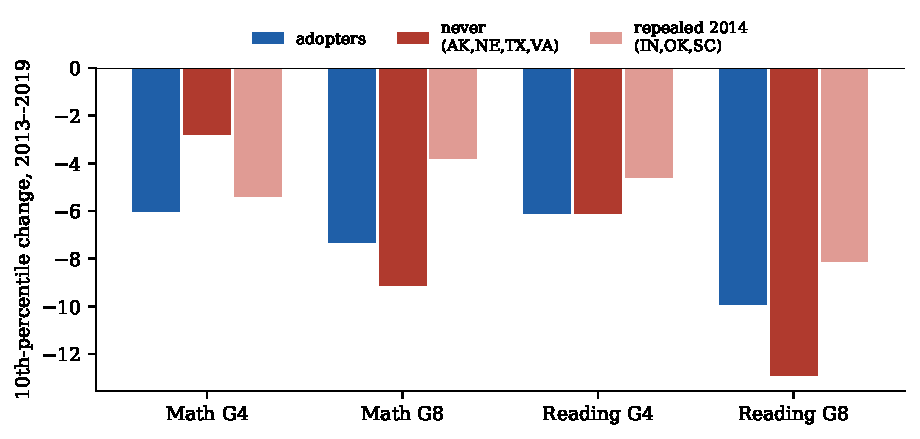
\includegraphics[width=.78\textwidth]{fig_commoncore.pdf}
\caption{10th-percentile score changes, 2013--2019, by Common Core adoption status. Data: NAEP Data Service API; adoption coding from NCES State Education Reforms.}
\label{fig:cc}
\end{figure}

\subsection{4G rollout timing: no detectable effect on the arrival-timing margin}
\label{sec:fourg}

If the saturation of adolescent life by smartphones and digital media drove the decline, the infrastructure rollout that carried it supplies a test of the same kind: counties crossed into high-speed mobile coverage at different times, and scores should have begun falling where and when 4G arrived. This section runs that test as an adversarial check on the report's own leading candidate, pointing the fertility literature's identification strategy (Section~\ref{sec:h2}) at test scores. Using the archived National Broadband Map (block~$\times$~provider mobile coverage, nine semiannual waves spanning the entire 2010--2014 LTE rollout, validated against FCC benchmarks, Verizon's December 2010 launch markets, and the later Form 477 data), we construct each county's high-speed-mobile coverage history and define treatment as the first wave in which coverage passes half the county's population. Matched to SEDA~5.0 county means (grades 3--8, mathematics and reading, 2009--2019; 99.9\% of counties merge), this is, to our knowledge, the first within-U.S. mobile-rollout design run against student achievement. The identifying variation is the rural lag: metro counties typically crossed the threshold around 2011--2012, nonmetro counties one to three years later. The design identifies one margin: whether a county's local 4G arrival timing moved its students' scores, relative to counties not yet or never covered. It is the direct rollout-variation test the digital-media hypothesis invites.

The result is a precise null on the arrival-timing margin, in both the contemporaneous-dose and exposure-year designs (Figure~\ref{fig:fourg}). The contemporaneous dose coefficient, moving a county from zero to full LTE coverage, is $-0.002$ SD (cluster SE $0.004$; permutation $p=0.66$); a within-county-year design identifying from cross-grade differences in adolescent exposure yields $+0.011$ SD per exposed year (permutation $p=0.12$). A ten-specification robustness grid (alternative speed-tier codings, Verizon-only coverage, 25\%/75\% thresholds, dropping five states with known coverage-coding artifacts, unweighted) keeps every coefficient within $\pm0.003$ SD, with signs that flip across specifications. The test is informative, not merely underpowered. The 80\%-power minimum detectable effects are $0.013$ SD on the dose margin and $0.016$ on the exposure-year margin, several times smaller than the $0.04$--$0.08$ SD effects \citet{jainstemper2024} estimate on the cross-country 3G margin. The only nominally significant patterns (a small \emph{positive} drift for early-treated counties, reading-only, growing with time since treatment) are continuations of a visible pre-trend, carry the wrong sign for the harm hypothesis, and disappear when the artifact states are dropped: the signature of mildly diverging urban--rural trends, the design's flagged first-order threat, not of a treatment effect.

What the null rejects is the strong local form of the hypothesis, in which the arrival of high-speed mobile infrastructure in a county drove its students' scores downward. What survives by construction is the national form: if the operative exposure was the device's saturation of adolescent social life, spreading on existing networks and synchronized nationally, it hit all counties in the same years, is absorbed by the year fixed effects, and is invisible to this design. Two further limits narrow what the null prices. Smartphone adoption ran substantially on existing 3G networks (teen ownership was already 37\% in 2012), so coverage timing is a noisy and partly anticipated instrument for exposure. And controls are exhausted by 2015 (the never-treated remainder is 117 deep-rural counties, half a percent of population), so slowly accumulating effects materializing four or more years after arrival are outside the design's reach. This is the same two-form reading the waiver test imposes on the accountability hypothesis (Section~\ref{sec:waiver}); neither leading candidate is exempted from it. What the null establishes is still informative on its own terms: the decline did not propagate through differences in when high-speed mobile infrastructure arrived, in instructive contrast to teen fertility, where the same variation produces large effects \citep{hudsonmoscoso2026}. Whatever digital media did to American adolescents' learning, it arrived with the device and its saturation of social life, not with the local cell tower upgrade.

\begin{figure}[tbp]
\centering
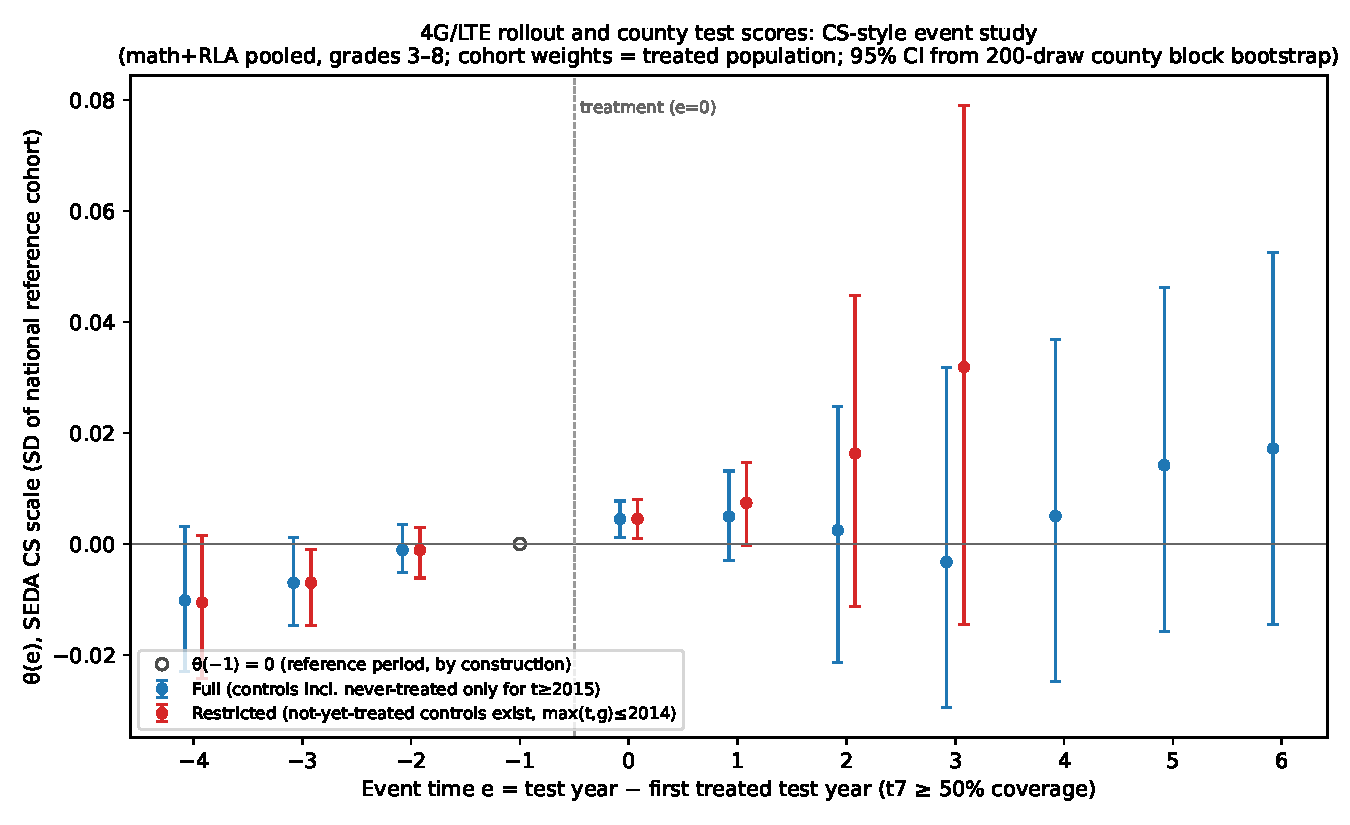
\includegraphics[width=.8\textwidth]{fig_4g_eventstudy.pdf}
\caption{Event study of county 4G (LTE) arrival on SEDA county test scores, pooled grades 3--8, mathematics and reading, 2009--2019. Cohort-weighted ATT$(g,t)$ aggregates by event time, with county-block-bootstrap 95\% CIs; the restricted series uses only comparisons for which not-yet-treated controls exist. Treatment is the first wave in which county high-speed mobile coverage exceeds 50\% of the county's population (NBM/SBDD archive). Units: SEDA cohort-standardized (SD) scale.}
\label{fig:fourg}
\end{figure}

\subsection{What the tests jointly imply}

The five tests hold the two leading hypotheses to one standard, and the two timing designs return the same kind of result. The waiver test rejects the strong local form of the accountability hypothesis: a state's formal release from NCLB consequences did not move its bottom decile, in a design powered to detect well under half the effect size accountability is credited with creating (Section~\ref{sec:waiver}). The 4G test, which this project ran as an adversarial check on its own leading candidate, rejects the strong local form of the digital-media hypothesis: a county's high-speed-mobile arrival did not move its students' scores, with minimum detectable effects several times below the cross-country 3G estimates (Section~\ref{sec:fourg}). The Common Core test does the same to a third policy candidate: states that never adopted the standards declined as much as adopters (Section~\ref{sec:commoncore}). In each case what survives, by construction, is a nationally synchronized channel that year effects absorb. Neither leading hypothesis leaves this section with a demonstrated local channel.

What still separates the two is positive evidence, not survival of elimination: the adolescent-period incidence of the losses (Section~\ref{sec:cohort}), the sector-neutral reading decline (Section~\ref{sec:sector}), the recurrence across rich countries and among PIAAC adults (Section~\ref{sec:adults}), and the coincidence with collapsing voluntary reading and with device-engagement gradients concentrated where the losses are (Section~\ref{sec:h2}) are each facts the digital-media hypothesis predicts and the school-policy hypotheses do not, standing independently of any elimination argument. The accountability retreat survives in a weaker form: a national climate change contributing through channels common to all states, with its clearest remaining footprint at the public-school grade 4 bottom decile.

Two boundaries keep this conclusion honest. First, the digital-media hypothesis faces direct policy variation of its own: the quasi-experimental ban literature \citep{belandmurphy2016,abrahamsson2024,beneito2022,figlio2025}, whose test-score gains concentrate among previously low-achieving students, and the pre-registered test of staggered U.S. state phone bans against NAEP 2026, specified in this project's repository in advance of the data. That pairing is the smartphone-side analog of the waiver test: the same design logic pointed at the other leading hypothesis. Second, elimination arguments are only as strong as the candidate list, and the list stays open. The hypotheses examined here are the ones prominent in research and public debate, not a partition of all possible causes, and a rival not on the list is untouched by the failures of those on it. The strongest claims in this report are accordingly its rejections; the ranking among the surviving candidates is stated in Section~\ref{sec:synthesis} in those calibrated terms.

\section{Channel Checks: Schooling Mode and Attendance}
\label{sec:mechanism}

The tests of Section~\ref{sec:sharper} discriminate between explanations for phase one; this section turns to phase two and to measurement. Two analyses probe the channels behind phase two directly: merging state NAEP changes with measured pandemic schooling mode, and exploiting NAEP's own student-reported attendance data. A third subsection asks whether the measured decline could instead be an artifact of falling test-taking effort.

\subsection{Schooling mode: the district-level effect mostly washes out between states}
\label{sec:dose}

Between-state variation in pandemic schooling mode explains almost none of the between-state variation in NAEP score declines. The treatment measure comes from the COVID-19 School Data Hub's district learning-model records, aggregated to enrollment-weighted state shares (47 states plus DC; Iowa, Montana, and Oklahoma are uncovered). In a regression of states' 2019--2022 NAEP changes on the share of the 2020--21 school year spent fully virtual, the relationship is right-signed but weak in mathematics ($-0.33$ points per 10 percentage points virtual at grade 4, $p=0.13$; $-0.18$ at grade 8, $p=0.35$), absent in reading (grade 8 is wrong-signed), and essentially zero pooled across the four series ($-0.04$ points per 10pp, $p=0.80$, clustered by state); Figure~\ref{fig:dose} (left) shows the grade 4 mathematics scatter. (The right panel plots the companion association: states' 2019--2024 net changes against their rise in chronic absenteeism.) The result is robust to excluding DC and, if anything, strengthens under enrollment weighting (weighted slopes are zero in mathematics).

\begin{figure}[tbp]
\centering
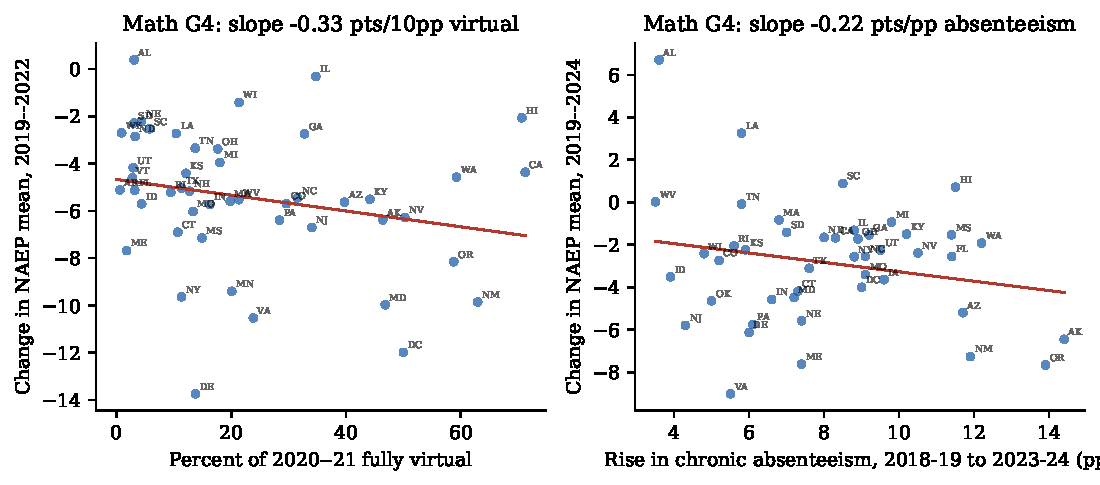
\includegraphics[width=.95\textwidth]{fig_doseresponse.pdf}
\caption{State dose-response. Left: change in grade 4 mathematics, 2019--2022, against the enrollment-weighted share of the 2020--21 school year spent fully virtual (COVID-19 School Data Hub). Right: net change 2019--2024 against the rise in chronic absenteeism, 2018-19 to 2023-24 (FutureEd state tracker).}
\label{fig:dose}
\end{figure}

The same exercise pushed below the state level, to NAEP's Trial Urban District Assessment, again finds only a weak dose-response (Figure~\ref{fig:tuda}). The 26 TUDA districts span essentially the full treatment range (Dallas, Miami-Dade, and Hillsborough were near-fully in person; Atlanta and Philadelphia fully virtual), and each is matched here to its own CSDH district record. Even with that contrast, the gradient in NAEP is weak: $-0.29$ to $-0.34$ points per 10pp virtual at grade 4 ($p\approx0.12$--$0.16$), zero at grade 8, $-0.18$ pooled ($p=0.23$), and no relationship between virtual share and 2019--2024 net change. The confidence intervals are wide enough to admit effects of the size the growth-based literature reports. The right reading is therefore not contradiction but limitation: NAEP's cross-sectional district samples (with standard errors of 1.5--2.5 points) and the restricted, all-urban TUDA sample blur a gradient that longitudinal growth data resolve.

\begin{figure}[tbp]
\centering
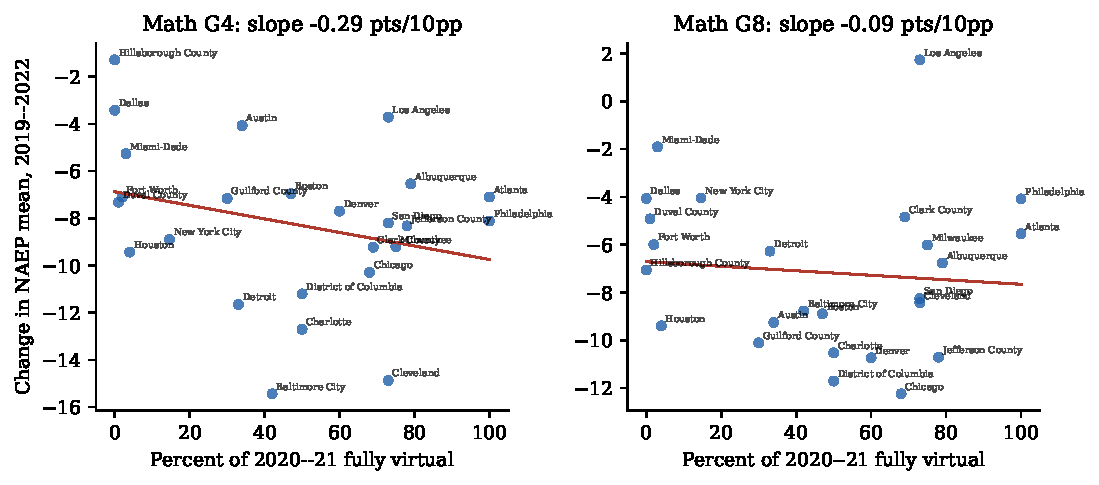
\includegraphics[width=.95\textwidth]{fig_tuda.pdf}
\caption{TUDA district dose-response: change in NAEP mathematics means, 2019--2022, against each district's CSDH share of 2020--21 spent fully virtual.}
\label{fig:tuda}
\end{figure}

This state-level fact is not new, and it is not a refutation of the closure literature. It was observed when the 2022 scores were released \citep{barnum2022} and formalized by \citet{lsae2025}; the pooled estimate here confirms it. The district-level studies \citep{goldhaber2023,jack2023} exploit far larger within-state treatment variation with apter controls, and state aggregation compresses both the treatment (few states were mostly virtual on average) and the outcome (state NAEP changes carry sampling errors of roughly a point). The useful calibration is this: \emph{schooling mode explains the timing of the national 2019--2022 drop better than it explains which states fell most}. Factors that varied little between states (the disruption itself, the absenteeism surge, whatever was already eroding the bottom) dominate the state cross-section.

\subsection{Attendance: a pre-pandemic disengagement trend, visible inside NAEP}
\label{sec:attendance}

NAEP's own attendance item shows disengagement rising before the pandemic, earlier than administrative records indicate. The assessment asks students how many days of school they missed in the month before the assessment, providing an attendance measure tied directly to scores and consistent since 2002. Three facts emerge (Figure~\ref{fig:absence}). First, the share reporting three or more missed days sat in the 19--22\% range from 2003 through 2013 with no trend, then \emph{began rising before the pandemic}, reaching 24\% at grade 4 by 2019; it jumped to 32--35\% in 2022 and remained near 30\% in 2024. This mirrors the administrative chronic-absenteeism record \citep{malkus2025} while revealing a disengagement pre-trend that the administrative data (flat at $\sim$15\% through 2019) understate. Second, the score penalty associated with absence widened sharply \emph{before} COVID: the gap between students missing no days and those missing more than ten grew from 29 to 42 points in grade 8 reading between 2013 and 2019. Absence became more academically costly, or increasingly selected the most disengaged students, exactly when the bottom of the distribution was collapsing.

Third, a Kitagawa decomposition splits each mean change into the part from students shifting into higher-absence categories and the part from score declines within categories. The absence shift accounts for roughly 25--42\% of the 2019--2024 declines (e.g., 42\% in grade 4 mathematics, 25\% in grade 8 mathematics), closely bracketing the Council of Economic Advisers' estimate, but for only 7--19\% of the pre-pandemic grade 8 declines. Phase one was not an attendance phenomenon.

\begin{figure}[tbp]
\centering
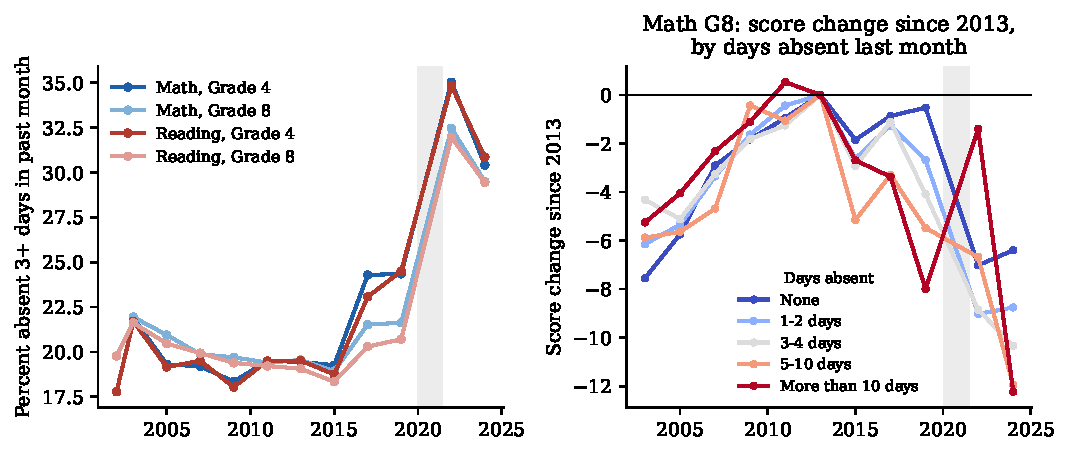
\includegraphics[width=.95\textwidth]{fig_absence.pdf}
\caption{Student-reported absence inside NAEP (B018101). Left: share reporting 3+ missed days in the month before the assessment. Right: grade 8 mathematics score changes since 2013 by absence category. Data: NAEP Data Service API.}
\label{fig:absence}
\end{figure}

The decomposition is associational (absence proxies broader disengagement), but the pattern coheres with everything above: phase one operated through something other than attendance; phase two converted a disruption into a persistent attendance and engagement problem that the recovery has not closed.

\subsection{Test-taking effort: a real wedge in levels, too small to explain the decline}
\label{sec:effort}

A remaining measurement alternative deserves a direct check rather than a footnote: perhaps students did not lose skill but stopped trying. NAEP, PISA, and PIAAC are all low-stakes for the test-taker, and effort demonstrably matters for their \emph{levels}: a surprise monetary incentive raised U.S. high-schoolers' scores on PISA-style items by roughly a quarter of a standard deviation (with no effect in Shanghai) \citep{gneezy2019}; incentives raised grade 12 NAEP-style reading scores by at least 5 points \citep{braun2011}; and effort proxies explain a third of cross-country PISA variation \citep{zamarro2019}. If students simply began trying less hard after 2012, part of the measured decline could be motivational rather than cognitive.

Three pieces of evidence bound the concern. First, PISA's ``effort thermometer'' asks students to rate (1--10) the effort they invested and the effort they would have invested had the test counted, in both 2018 and 2022. In the microdata, reported effort fell by just 0.13 points in the U.S. and 0.16 across the OECD; multiplying by the cross-sectional effort--score gradient (3.9 points per effort point, ESCS-adjusted, itself an upper bound on the causal effect) implies an effort-attributable change of roughly \emph{half a point} of the 13--15-point 2018--2022 PISA decline, under five percent. Second, the OECD's behavioral indicators move the wrong way for an effort story. The within-test fatigue gap (first vs.\ second hour) \emph{narrowed} in 2022, meaning scores fell most at the \emph{beginning} of the test; answer straight-lining declined; and the OECD concluded that administration conditions ``remained similar,'' singling out only Albania \citep{oecd2023}. Rapid-guessing prevalence across countries is essentially uncorrelated with mean performance \citep{avvisati2024}, and no NCES analysis documents rising disengaged responding on digital NAEP. Third, and decisive for the U.S. case, the same 2013--2019 decline appears where the motivation story cannot follow it. It shows up in \emph{state accountability tests}, which carry stakes for schools: the SEDA archive of roughly 70 million students' consequential state assessments \citep{dewey2026}. And it shows up among PIAAC adults, where the school-test motivation dynamic does not apply.

A caution survives. Across countries, the change in even \emph{hypothetical} (``if it counted'') effort correlates 0.64 with the change in mathematics performance, so motivation and measured skill co-move, most plausibly because both are downstream of the same disengagement that the absence and reading-practice data record. The honest conclusion is that effort is a real wedge in score \emph{levels}, but the change in effort is far too small to explain the decline. To the extent motivation has eroded, it is part of the phenomenon, not an artifact contaminating it.

\section{Synthesis: A Two-Phase Decline With Different Causes}
\label{sec:synthesis}

\begin{table}[tbp]
\centering\footnotesize
\caption{Hypothesis scorecard: consistency of each candidate explanation with the facts of Section~\ref{sec:verify}.}
\label{tab:scorecard}
\begin{tabular}{lcccccc}
\toprule
 & F1 & F2 & F3 & F4 & F5/F7 & F6 \\
Hypothesis & Timing & Bottom-heavy & COVID drop & No recovery & Within-group & Intern'l \\
\midrule
H1 Pandemic            & $\times$ & $\sim$ & \checkmark & $\sim$ & \checkmark & $\sim$ \\
H2 Digital media       & \checkmark & $\sim$ & $\times$ & \checkmark & \checkmark & \checkmark \\
H3 Accountability      & \checkmark & \checkmark & $\times$ & $\sim$ & \checkmark & $\times$ \\
H4 Funding cuts        & $\sim$ & $\times$ & $\times$ & $\times$ & $\sim$ & $\times$ \\
H5 Demographics        & $\times$ & $\times$ & $\times$ & $\times$ & $\times$ & $\times$ \\
H6 Absenteeism         & $\times$ & \checkmark & \checkmark & \checkmark & \checkmark & $\sim$ \\
H7 Reading practice    & \checkmark & $\sim$ & $\times$ & \checkmark & \checkmark & \checkmark \\
H8 Teachers/inflation  & $\sim$ & $\sim$ & $\times$ & $\sim$ & $\sim$ & $\times$ \\
H8 Mental health       & \checkmark & $\sim$ & $\times$ & \checkmark & \checkmark & \checkmark \\
\bottomrule
\multicolumn{7}{l}{\footnotesize \checkmark{} = consistent; $\sim$ = partially consistent; $\times$ = inconsistent or silent.}\\
\multicolumn{7}{l}{\footnotesize Consistency is a screen, not a causal attribution (direct tests: Sections~\ref{sec:sharper} and~\ref{sec:mechanism});}\\
\multicolumn{7}{l}{\footnotesize the identical H2 and mental-health rows are separated only by evidence outside the table (Section~\ref{sec:h8}).}
\end{tabular}
\end{table}

A useful discipline can be borrowed from the parallel debate over collapsing birth rates, which shares this puzzle's structure: a synchronized post-2010 break across rich countries that resists every standard policy explanation \citep{kearneylevine2022,evans2024}. A candidate cause must clear two bars \emph{simultaneously}. It must explain the synchrony (the same decline appearing across countries with disparate school systems, funding trends, and accountability regimes, and among adults no school policy touches), and it must explain the local signature: bottom-of-distribution concentration, adolescent-period timing, sector neutrality. Every school-policy explanation fails the first bar by construction; the pandemic fails the second for phase one, having arrived six years late. Two candidates examined here clear both bars, the second in its adolescent form: digital media (H2) and the deterioration in adolescent mental health (Section~\ref{sec:h8}), rivals that the causal literature itself entangles and that differ mainly on whether devices are the cause or a covariate of the distress rise. The ban studies, in which removing devices improves achievement and mental health together, favor the first reading, but nothing in this report's evidence eliminates the second. With that framing, the evidence is not consistent with any single-cause account, but it is well organized by a two-phase model (Table~\ref{tab:scorecard}):

\textbf{Phase one (2013--2019): erosion at the bottom.} Slow national decline, concentrated almost entirely among the lowest-performing students, present in most states and many countries, alongside collapsing voluntary reading. Two hypotheses fit these basic facts most directly: the accountability retreat (which predicts the bottom-concentration and the U.S. policy timing, and is corroborated in mirror image by Mississippi) and digital-media displacement (which predicts the international synchrony and the reading-practice collapse). The timing tests of Section~\ref{sec:sharper} reject the strong local form of each, using each hypothesis's own variation: release from NCLB did not move a state's bottom decile, and 4G arrival did not move a county's scores. What ranks digital media ahead is positive evidence rather than survival of elimination; Section~\ref{sec:sharper} assembles it, and Section~\ref{sec:adults} extends it to adults. On this evidence digital media is the best-supported remaining candidate for phase one, not an established cause, and the pre-registered 2026 state-ban test is the next direct check.

The accountability retreat retains a plausible supporting role (as a national climate shift, and at the public-school grade 4 bottom decile, where the sector contrast does point its way), but the strong version in which deregulation drove the floor down is rejected by its own state-level test. Funding, demographics, and teacher supply fail on timing, distribution, or magnitude.

\textbf{Phase two (2019--2024): shock without recovery.} The pandemic caused the large 2019--2022 drop (the schooling-mode dose-response evidence is decisive) and hit the whole distribution. What demands explanation is the aftermath. Four-plus years on, aggregate recovery is negligible, reading is still falling, and among adolescents the bottom decile continues to sink while the top rebounds; the 2025 LTT shows the first exception, a bottom-led rebound among 9-year-olds, while 13-year-olds remain stuck. Persistently doubled chronic absenteeism is the leading proximate cause, with the phase-one forces (weak accountability pressure, screen displacement) plausibly explaining why disengagement has not self-corrected.

The magnitudes in Table~\ref{tab:changes} put the two phases in proportion: phase one accounts for roughly 20--46\% of the total 2013--2024 decline depending on the series, and the pandemic window for most of the rest: from 28\% in grade 8 reading, where the pre-pandemic slide dominated, to more than the entire net total in grade 4 mathematics, where post-2022 gains offset part of the pandemic drop. Even a complete reversal of pandemic losses would therefore leave the United States well below its 2013 peak.

\section{Limitations}

This analysis is observational. The hypothesis tests rest on timing, distributional incidence, and cross-sectional comparisons, not experimental variation. Several causes plausibly interact (absenteeism is partly downstream of screens and of weakened school engagement), so the phase shares above are accounting decompositions, not causal attributions.

The data series themselves carry known measurement caveats. NAEP percentile statistics for the oldest years use no-accommodation samples; the NSLP-eligibility series ends in 2022 and is affected by community-eligibility expansion; PISA OECD averages shift membership across cycles; and PIAAC cross-cycle comparisons involve assessment changes and should be read as NCES advises. The LTT format changed in 2004 (results are bridged). The 2025 LTT wave is reported from Data Service point estimates whose standard errors are not yet published in the Digest, so significance language for 2023$\rightarrow$2025 changes follows the NCES release. Measurement artifacts, by contrast, can be largely ruled out as an explanation of the decline itself: NAEP exclusion rates were flat at 1--3\% of all students from 2013 through 2024 even as SD/EL identification rose; student participation was identical in 2022 and 2024 (92\% at grade 4, 89\% at grade 8); and public-school participation was complete. Neither rising exclusion nor falling participation can explain the declines; grade 12, with 68\% student participation in 2024, is the exception and is treated cautiously.

The report's own tests (Sections~\ref{sec:sharper} and~\ref{sec:mechanism}) carry design caveats. In the waiver analysis, the never-waiver comparison group is seven states, so inference uses randomization rather than cluster asymptotics and the minimum-detectable-effect calculation bounds what the null can claim; pre-2011 trend differences are visible ($p=0.08$ jointly); and waivers capture only the formal step of deregulation. The 4G-rollout test is informative only about local arrival timing and has imperfect pre-trends. Neither timing design can see a nationally synchronized change: a national accountability climate and a national adoption wave alike are absorbed in year effects. Catholic-school samples are small and selected, so only their trends, not their levels, are informative, and only the reading trends are estimated precisely enough to discriminate. The schooling-mode state regressions are aggregation-limited: state-level treatment variance is a fraction of district-level variance, and three states lack schooling-mode data. NAEP's absence item covers only the month before the assessment, and the Kitagawa decomposition treats absence as exogenous when it partly proxies disengagement.

Finally, the digital-media evidence is a composite, and each component carries limits of its own. The PISA distraction and screen-time gradients are cross-sectional associations: low performance may drive device retreat as well as the reverse, and the leisure-hours items were not administered to U.S. students. The quasi-experimental ban literature is small, though consistent. The rollout-based causal designs concern outcomes that are either non-U.S. test scores or non-achievement domains (fertility, mental health). The causal magnitudes at the population scale of the U.S. decline therefore remain uncertain, and the adult PIAAC comparison carries its own caveats beyond the cross-cycle caution noted above: a 28\% U.S. response rate in 2023 and a change to tablet-only administration. The adolescent mental-health rival added in Section~\ref{sec:h8} is acknowledged rather than resolved: the rollout and ban literatures entangle the distress rise with the device shock in both directions, and nothing in this report's data identifies whether devices are cause, joint product, or mere covariate of deteriorating adolescent mental health.

\section{Verification}
\label{sec:verification}

This report was produced by a language-model agent (Claude Fable 5) directed and verified by the author. That division of labor raises a legitimate reliability question: the volume of data work involved (dozens of API pulls, fourteen analysis scripts, hand-coded policy datasets, two-gigabyte microdata files) exceeds what any reader, including the author, can efficiently audit line by line. Rather than asking for trust, the project carries a layered verification record, all of it in the public repository alongside the code and data (\url{https://github.com/brendanbartanen-svg/naep-achievement-decline}).

\textbf{Claims audit.} Every load-bearing claim in this report (44 in total) is cataloged in \texttt{evidence/claims\_audit.md} and typed by provenance: 13 are \emph{citations} to published work (no trust in this project's code required), 3 are \emph{pulled} federal statistics, and 26 are \emph{computed} here. Each row carries a verification path executable in under five minutes---a NAEP Data Explorer navigation, a Digest of Education Statistics table number, or the cited paper's table. The audit also identified the report's one provenance gap: the LTT percentile changes for waves through 2023 are hand-transcribed from Digest tables 221.85/222.85 rather than recomputed from raw data, so external table checks, not code review, are their verification. (The 2025 wave does not share this gap: its means and percentiles were pulled directly from the LTT Data Service, with the extraction recorded in \texttt{evidence/ltt\_2025.md} and frozen in \texttt{checks.py}.)

\textbf{Assertion suite.} A test script (\texttt{checks.py}, 71 assertions) recomputes the headline descriptive facts from the raw data files---peak years, the 2024 records, the 90--10 gaps, the sector changes---and freezes every computed result against its stored value, so that any subsequent change to code or data that silently moves a published number fails loudly. The suite runs clean on the version of record.

\textbf{Blind clean-room replication.} The five computed results judged most error-prone were independently re-derived by separate agents that were denied access to this project's analysis code, results files, and text, and instructed not to search for the answers. Each re-pulled the data from the NCES API or read the raw PISA files directly. All five reproduce. The cohort decomposition matched to the decimal ($-4.45 = +1.57 - 6.02$ against the published $-4.4 = +1.6 - 6.0$). The PISA distraction estimate matched exactly for the U.S. ($-13.25$ vs.\ $-13.2$), and the replicating agent independently recovered the counterintuitive item coding (1 = ``every lesson'') from the file's own metadata, precisely the step where a sign error is most likely. The Kitagawa inputs matched to the decimal, and the decomposition shares fell inside the published bands. The Catholic-sector changes matched exactly, with NAEP's official significance tests agreeing with every conclusion published here. The waiver analysis reproduced the null and the informative MDE while showing that the near-zero point estimate is window- and pooling-dependent, which is why it is reported as $\approx$0 rather than as a precise value. No pipeline errors were found; every divergence traced to a documented convention choice (weighting, window, or standard-error construction). The full comparison is in \texttt{verification/cleanroom/COMPARISON.md}.

\textbf{External anchoring.} Where this report's computations overlap independently published estimates, they agree: the waiver null corroborates \citet{bleiberg2020}; the state-level schooling-mode non-result is consistent with how the district-level closure effects of \citet{goldhaber2023} and \citet{jack2023} aggregate; the PISA gaps track the OECD's published bivariate versions \citep{oecd2024}; and the 4G exposure panel of Section~\ref{sec:fourg} was validated against FCC-published coverage benchmarks and Verizon's documented December 2010 launch markets before any outcome data were attached.

\textbf{Human verification.} The components that machine verification cannot reach were checked by the author. The four hand-coded policy datasets (waiver dates, phone-ban statutes, Common Core adoption status, and the TUDA--CSDH crosswalk) were spot-checked against primary documents, with attention to the rows where a coding error would change treatment assignment; the five headline NAEP numbers were re-pulled manually from the Data Explorer; and the Synthesis section was reviewed adversarially by an independent colleague. The residual risks are stated rather than hidden: the interpretive weighting of Section~\ref{sec:synthesis} is a judgment no audit can certify, and the pre-registered NAEP 2026 phone-ban test is how the project lets future data discipline it.

\section{Conclusion}

The decline in American student achievement is real, large, and verifiable from primary data: roughly one grade level of learning lost at grade 8 since 2013, the lowest grade 8 reading scores ever recorded, and the widest achievement gaps in NAEP's history. It happened in two phases with different causes. The pre-pandemic erosion, nearly invisible in averages because it was confined to the bottom of the distribution, points to a post-2012 transformation of adolescent life in which smartphones and digital media are the better-evidenced driver and deteriorating adolescent mental health an entangled companion these data cannot separate; the evidence behind that ranking is assembled in Sections~\ref{sec:sharper} and~\ref{sec:synthesis}, and the pre-registered state phone-ban test against NAEP 2026 is the next opportunity to corroborate or overturn it. The retreat from test-based accountability likely contributed at the margins, most visibly at the public-school grade 4 bottom decile, but failed the direct tests this report could put to it. The pandemic then imposed the largest schooling shock in modern history, whose effects, far from fading, have been locked in by chronic absenteeism that remains half again its pre-pandemic level. Funding cuts, demographic change, and teacher shortages are, on the evidence, second-order.

Three implications follow. First, ``COVID recovery'' framing understates the problem: grade 8 reading was already down 4.4 points before the pandemic, and the forces behind that slide are still operating. Second, because losses are concentrated at the bottom, average-score targets understate the equity emergency; the 90--10 gap is the widest ever measured. Third, with the school-policy explanations weakened by the tests of Section~\ref{sec:sharper}, the empirical frontier shifts to the digital-media hypothesis and its pathways, where causal evidence is accumulating: existing ban studies \citep{belandmurphy2016,abrahamsson2024,beneito2022,figlio2025} consistently find gains concentrated among low achievers, and the staggered adoption of U.S. state bans (roughly thirty states by 2025--26) against NAEP 2026 offers exactly the kind of test that waiver timing provided here; this project's repository pre-specifies the design and treatment coding. Mississippi's literacy reform remains the strongest evidence that aggressive instructional policy can buck the trend even if policy retreat did not cause it. The policy conclusion is uncomfortable but clear: returning to 2019 practices would only return the country to a trajectory that was already pointing down.

\bibliography{refs}

\end{document}
